%!TEX root = project.tex

\chapter*{About this project}
\paragraph{Abstract}
This project I developed as my final year project for the module Applied Project \& Minor Dissertation, the objective being to design a meal planning application using a MERN Stack (MongoDB, ExpressJS, ReactJS and NodeJS) where the application users should be able to register, log in, securing user accounts by encrypting user passwords, select meals to replicate, organize shopping lists, calculate BMR (Basic Metabolic Rate) and calories needed, and gather nutritional information on various diets.\\ \\
My aim with this project is to build a multi-user, functioning web application that is safe and secure following cyber security guidelines and presenting the user with a professional and fun User Experience. The project uses MongoDB to store and sexure all user information from the user sessions. The project should also provide an attractive and accommodating User Interface where the users can easily navigate through without difficulty.\\ \\
The goal I have with this project is to show the level of growth I have obtained as a Software Developer throughout my time in this course by learning and researching the depth of these technologies utilized. This project can be found in a GitHub Repository (there is a link in the Appendix section of this dissertation).

\paragraph{Author}
Hello, my name is \textbf{Emmanuel Osabuehien} (G00373559) and I am a Final Year student at Galway-Mayo Institute of Technology (GMIT).

\chapter{Introduction}

\section{Overview}

In this chapter, I will give a quick overview on my Introduction to my dissertation, where we will be going through some of the research conducted before the development of the application.\\ \\
Here I will be giving you insight into what my project is and why I decided to make this app.\\ \\
We will also be talking about the negatives and positives of most apps in my project field and the benefits of curating such an app.\\ \\
We will lastly be going through the software requirements that I plan to complete by the end of the apps developmental process.

\section {Meal Planning Application}

In this section, I will be giving a brief introduction into what my project is and why I have chosen to do it.\\ \\
My project is known as a Meal Planning System, this is a system that offers meals for people so they can plan and decide whats meet their dietary requirements and budget.

\begin{center}
  \begin{figure}[H]
    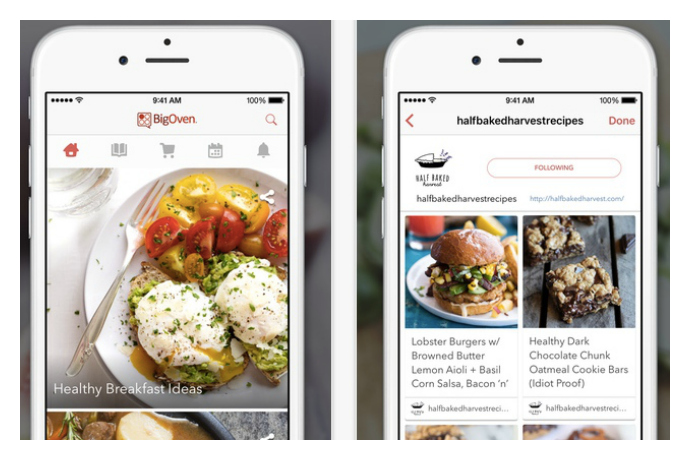
\includegraphics[width=\textwidth]{img/mealplanningpic.jpg}
    \caption{Mean Planning Example}
    \label{fig: Example of a Meal Planning System}
  \end{figure}
\end{center}

\subsection{What is a meal planning application?}

A meal planning application is an app that you plan several weeks of meal plans/grocery lists and then put those weekly meal plans into a rotation, this system is designed for users to eat healthier, giving users the decision to think about what they would like to eat and will those select items provide your body with nourishment.

\subsection{History of meal planning}

First, time devoted to cooking has decreased: in the United States, it has been reduced from 1:63 hour per day in 1965–1966 to 58 min in 2006–2007. Additionally, the source of food consumed has changed: people consume less food prepared at home, whereas foods prepared away from home represent an increasing part of the diet. These studies highlighted that the consumption of food prepared away from home is associated with a lower quality diet and a higher body mass index, whereas benefits have been attributed to home-prepared food. \\ \\
Previous research emphasized that individuals with lower cooking skills were more likely to consume away from home food such as ready meals or take-out meals from fast food or restaurants. To face time pressure, a series of qualitative studies highlighted that parents resort to food choice coping strategies, such as meal simplification, taking out, or meal planning despite their potential impact on diet quality. \\ \\
Among these strategies, time management skills and in particular meal planning, which consists in deciding ahead the foods that will be eaten in the next few days, has been previously suggested as a solution to balance competing time demands and reduce barriers to healthy dietary practices. Studies performed on general populations showed that meal planning was positively associated with frequencies of home food preparation and family meal, as well as the presence of fruits for dinner. \\ \\
In the present study, we hypothesize that meal planning might encourage home meal preparation, and therefore have beneficial effects on dietary quality and consequently on weight status. Then, we investigated the relationships between meal planning and diet quality, based on adherence to nutritional guidelines, energy, macronutrients and food group intakes, as well as food variety.

\subsection{Why am I making meal planning system?}

Q. Why have I choose an meal planning system? \\ \\
A. I believe this is completely correct in scope for my a software project as can conjure up many queries for me as a developer, examples of this may be how can I protect user information and how can I create a functional customer to supplier relationship within this software. This line of questioning is necessary as it is a much needed addition as I gain experience as a developer. I believe that this application is great as a developer as I gain a understanding from both a perspective of both a developer and user and some of the issues both can face. This application will enhance the skills all software developers should have time management, cross-platform software, database knowledge and problem solving. This type of application is needed for a variety of different users, for example myself as a student living away from home, I have now work independently and try provide for myself which is hard due to not always having to fund to go out and buy a vast amount of ingredients, this app can help from young people, people with deficiencies, people planning to lose wight, etc. with these sorts of issues.

\subsection{What are some of my issues with most meal planning systems and how do I think they can be improved?}

Many users of a typical meal planning systems depending on who you ask tend to have many problems with many modern meal planning apps, this can include apps such as 'Paprika' and 'MealBoard'. Some of the problems I will discuss below and give my take on how to combat these issues \\ \\
\textbf{Lack of Information: }Many users of meal planning apps will tell you how their is a lack of information given to a regarding nutrients the body needs.
My plan to combat this is by presenting users with a graph that shows what is the percentage of food types necessary for a person to consume in a day. \\ \\
I will also present users with recipes/meals and proper instructions into how to prepare and cook these meals instead of just giving users a list of meals they would have to research by themselves.
\\ \\
\textbf{Practicality: }I aim to provide an eye-catching user interface by using the react libraries available such as React Bootstrap, ChartJS and React Hook Form to provide users with a simple meal planning app with a navigation bar to move through different pages and providing exciting features.\\ \\
\textbf{Lack of Customization: }I aim to make this app feel personal to the user, it will involving adding graph/charts showing expenditure towards meals giving the user a very different experience than what they are used to.\\ \\
\textbf{Economic Consideration: }Most apps regarding meal planning will not take into consideration users economic struggles, which is something I believe should be always kept in mind, to combat this issue I will provide a list of meals from cheap to expensive to make so users will not be worried about their expenditure when choosing meals. 
\\ \\
\textbf{User Interface: }The user interface on most meal planning apps are not easy on the eye and quite dull. I plan to make one of more quality and vibrant to visualize for a user so they are more intrigued when they view the app. \\ \\
These apps may also be difficult to understand how to move around, I plan to make my app so it will be a quite easy to for a new user to navigate around.

\section {MERN Stack}
In this section, I will be talking about a MERN Stack, we will be going through the points of what it is, why I am using it and how is it employed.
\begin{center}
  \begin{figure}[h!]
    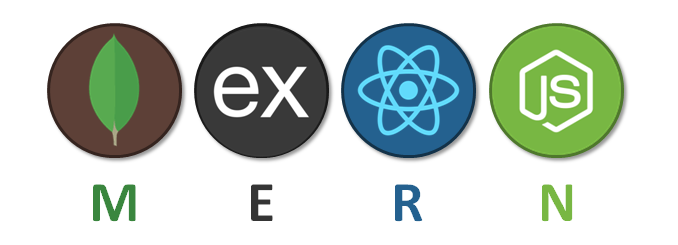
\includegraphics[width=\textwidth]{img/mern-stack.png}
    \caption{MERN Stack Logo}
    \label{fig: MERN Stack Image}
  \end{figure}
\end{center}
Now to put everything into context MERN is an acronym made up of the key technologies that make up the stack itself.
\begin{itemize}
\item M = MongoDB
\item E = ExpressJS
\item R = ReactJS
\item N = NodeJS
\end{itemize}
This is a big reason why I chose to use a MERN Stack for my project as this technology provides a smooth, simple way to make a full-stack web application that can be explained as follows. \\ \\
\textbf{MongoDB} is a open source, cross platform, NoSQL document-oriented database which is used to store a large amount of data in documents and collections. \\ \\
\textbf{ExpressJS} is server-side, back end web application framework that is used for NodeJS needed to write simple and secure applications. \\ \\
\textbf{ReactJS} is a open source, front end JavaScript Library used to create graphical user interfaces of web applications. \\ \\
\textbf{NodeJS} is a open source, cross platform back end JavaScript run time environment, running the JavaScript code outward of the browser. \\ \\

\subsection{MongoDB}

\begin{figure}[H]
  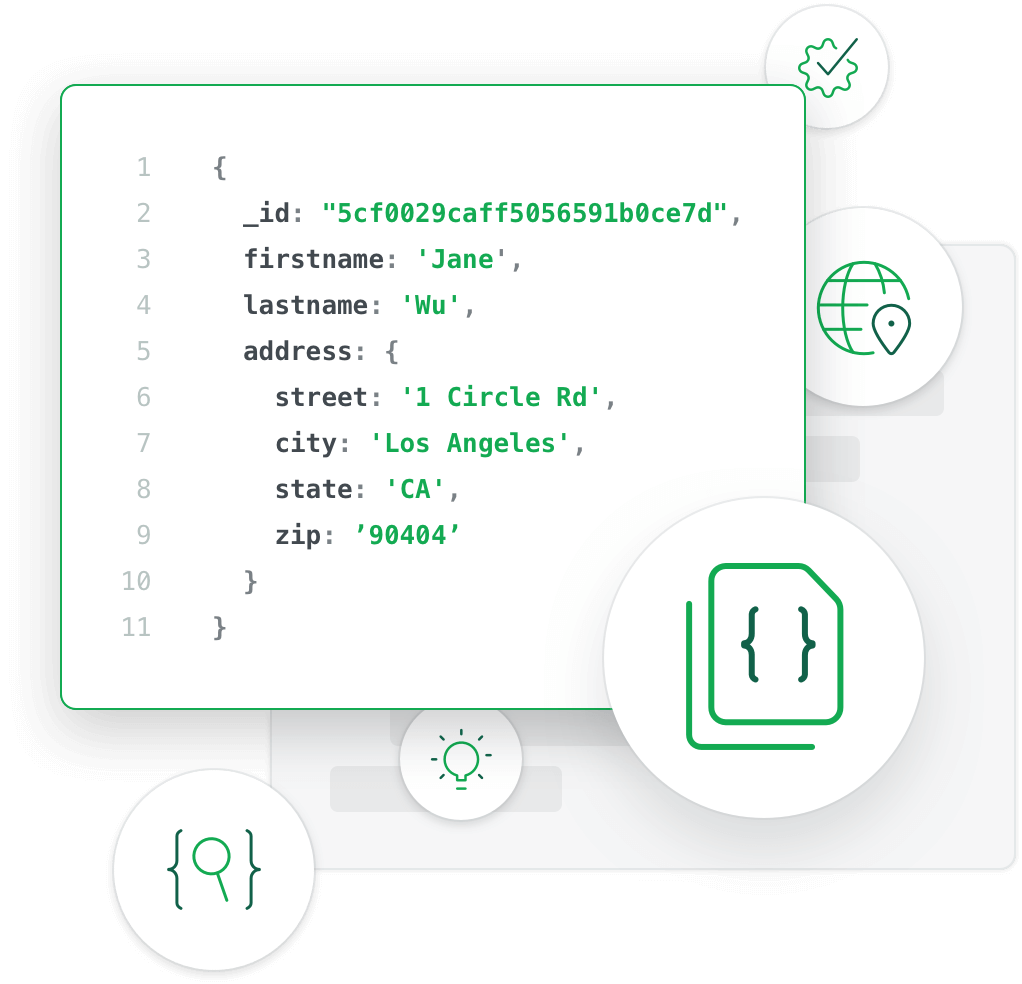
\includegraphics[scale=0.35]{img/mongodbeg.png}
  \centering
  \caption{Example of Mongo Database}
  \label{fig: Mongo Database}
\end{figure}

The reason I decided to use MongoDB as opposed to MySQL or other services available for my database management can be broken down into a couple of reasons, one of the big reasons is it's growth in popularity but removing that key factor MongoDB has many advantages over most services in this area including:

\begin{itemize}
\item\textbf{MongoDB} can handle large volumes of unstructured data
\item\textbf{MongoDB} has the ability to scale up quickly
\item\textbf{MongoDB} allows schemas to be flexibile due to it's data models
\item\textbf{MongoDB} is constantly evolving
\end{itemize}

\subsection{ExpressJS}

\begin{figure}[H]
  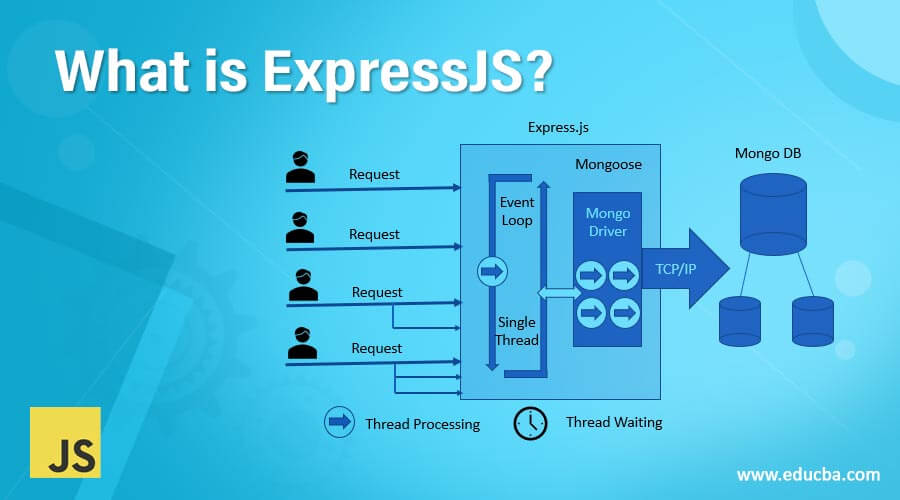
\includegraphics[scale=0.4]{img/whatisexpressjs.jpg}
  \centering
  \caption{Example of an ExpressJS process}
  \label{fig: What is ExpressJS?}
\end{figure}

The reason I chose ExpressJS as opposed to other frameworks for my back end development is due to it's high quality status of performing a server-side connection and it's ability for unfamiliar users to easily use, learn and understand, other positives include:

\begin{itemize}
\item\textbf{ExpressJS} allows users to use the same programming language as the front end
\item\textbf{ExpressJS} has the ability to scale your application quickly
\item\textbf{ExpressJS} can easily connect to databases such as MongoDB or MySQL
\item\textbf{ExpressJS} works well with NodeJS
\end{itemize}

\subsection{ReactJS}

\begin{figure}[H]
  
\includegraphics[scale=1.0]{img/reatcjspic.png}
  \centering
  \caption{Example of React App Symbol}
  \label{fig: React App Symbol}
\end{figure}

The reason I chose ReactJS as it is a JavaScript library that is great for building user interfaces and framework that has been on the rise since it's conception in 2013, ReactJS offers many services and features when creating an easy to navigate user interface, other advantages include:

\begin{itemize}
\item\textbf{ReactJS} is easy to use and understand
\item\textbf{ReactJS} provides reusable components of HTML code
\item\textbf{ReactJS} offers a scope where developer can test and debug code
\end{itemize}

\subsection{NodeJS}

\begin{figure}[H]
  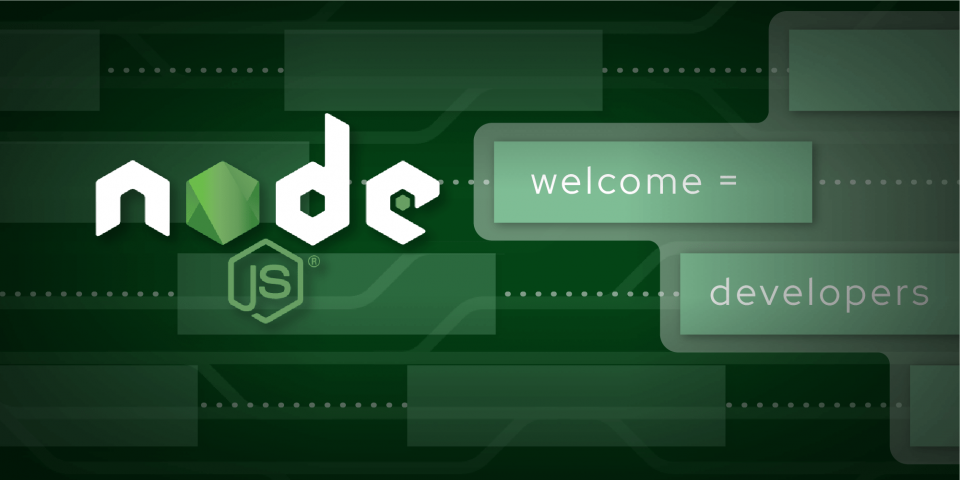
\includegraphics[scale=0.5]{img/nodejspic.png}
  \centering
  \caption{Image of NodeJS Background}
  \label{fig: NodeJS Background}
\end{figure}

The reason I chose NodeJS because it because of server-side security, what it also offers, which includes various tools and libraries useful in web applications and it's ability to easy handle server-side requests, other advantages include:

\begin{itemize}
\item\textbf{NodeJS} has the ability to scale up quickly
\item\textbf{NodeJS} is a very flexible run time environment
\item\textbf{NodeJS} is easy to use, learn and understand
\item\textbf{NodeJS} offers cross-platform development, for example you can connect a mobile app link to a desktop app
\end{itemize}

\section{Positives and Negatives of Meal Planning Systems}

In this section, I will discuss both the positives and negatives of meal planning applications

\subsection{Positives}

\begin{itemize}
\item Aiming for weight loss goals
\item Easy to prepare for shopping
\item Allows for better money management
\item Saves users time and energy
\item System offers users a wide variety of ideas to use
\item It might be able to offer some nutritional knowledge
\end{itemize}

\subsection{Negatives}

\begin{itemize}
\item Recipes may not be up to user satisfaction
\item It means setting a schedule and plan and sticking as close to it as possible
\item It takes planning and discipline to meal plan, that you might not have
\item Inflexible and don’t account for varying needs of the body
\end{itemize}

\section{The Benefits of Meal Planning Systems}

In this section, I will discuss the benefits of a meal planning application

\subsection{Health Goals}

 Cooking meals at home increases your chance of reaching health goals, whether or not they are planned to lose weight, improve heart health or keep blood sugar steady, meal planning is what gives you ingredients and resources to actually make this happen on a daily basis.

\subsection{Budgeting}

Meal planning makes it easier to cook more at home, and shoppers can save even more by weekly sales into planning. So the next time you're budgeting for an expense, consider meal planning to help save you money on a set basis.

\subsection{Enables Variety and Gives Control}

Meal planning is often associated with increased food variety, which is key to  a healthy diet that increases your goal of meeting nutritional needs.

Meal Planning also gives you control and choice over ingredients as it is easier to avoid food allergens and to incorporate ingredients that support diets for specific health problems

\subsection{Streamlines Shopping and Decreases Food Waste}

Meal planning allows users to set out their list of ingredients to obtain based around their meal plan, reducing the time and money spent to constant shopping trips.

You are also most likely to make use of forgotten food items that are just stored away, reducing the amount of food waste and unneeded shopping trips by utilizing what you already have on hand.

\subsection{Decision Fatigue}

Meal Planning helps to alleviate the stress and fatigue when deciding what to meals you need to make throughout the day as users can stock up ingredients and have multiple planned meals where they have a wide variety of options to choose from.

\section{Software Requirements}

In this section, I will give a list of the software requirements I intend my project to achieve

\begin{itemize}
\item\textbf{Login: }If user has an account, they are required to login to use application
\item\textbf{Register: }If users don't have an account, they are required to register an account and login to use application
\item\textbf{Logout: }Users can logout if application is not in use
\item\textbf{Forget Password: }If users can't access account/forgot their password, they can retrieve their account by following process provided
\item\textbf{Add Meal: }Uses can add meal into the listing page
\item\textbf{List All Meals: }Users can access listing page where they can view all meals that have been added
\item\textbf{Fetch Meal: }Users can retrieve the meal that they have added to the listing page
\item\textbf{Delete Meal: }Users can delete the meal that they have added to the listing page
\item\textbf{Edit Meal: }Users can update the meal that they have added to the listing page
\item\textbf{Cookies: }The application must use cookies to memorize information during visits and maintain sessions.
time-frame max of a day.
\item\textbf{Security: }Users login details must be encrypted and secure so they cannot be accessed by another user
\end{itemize}

\chapter{Context}

\section{Overview}

In this chapter, I will give a a more clear context on the contents of this document.\\ \\
We will go through the objectives that have been laid out and to be completed during the duration of development.\\ \\
I will briefly discuss each chapter in the document and the contents that each chapter contains.\\ \\
Finally, I will talk about how the project is structured in my GitHub repository including the files for this very document as well as the source files for the application. 

\section {Objectives}

In this section, I will discuss the key objectives that I intend to carry out for this web application. \\ \\
The objectives include:

\begin{itemize}
\item To create a multi-user, functioning web application that can be accessed
\item To an attractive, simple and easy to understand graphical user interface that users can operate without difficulty
\item To provide a system where users can plan out their meals
\item To provide users a system keep track of dietary goals
\item To provide users with nutritional education
\item To provide a multi-user app with a secure database of users where login details are encrypted
\item To provide a REST API to my service to allow users to perform requests
\end{itemize}

\section {Chapters}

In this section, I will give a brief overview of what each chapter in my dissertation contains.

\subsection{Introduction}

In this chapter, this is just an introduction of the project, where we what is the project, why I choose to make this project and use the technology I utilized, provides what are the key objectives of this project and give the viewer an idea on what this dissertation contains.

\subsection{Context}

As is evident by the title of this chapter, in this chapter I will discuss the context of my project, the importance and rise of web-based issue ticketing systems, the benefits and drawbacks of meal planning apps and how convenient they came to be in modern computer science especially in a software project collaborative setting.

\subsection{Methodology}

In this chapter, I will discuss my approach to this project, the methodology and testing I used for this project and why I chose a certain type of methodology and testing, how this had an effect on my project and go into more detail on how the developmental process of my project

\subsection{Technology Review}

In this chapter, I will discuss more about the technical features of the project, all the technologies used in my project at a more conceptual level, how did they affect the developmental process, why did I choose this technology to implement and should a good indication of the research that was undertaken during the creation of the project.

\subsection{System Design}

In this chapter, I will give a detailed explanation of the system architecture i.e., Front End, Back End, Database. There will be an overview of the different components of the system and how they function together when deployed and diagrams to explain and visualize the design of the system.

\subsection{System Evaluation}

In this chapter, I will give an evaluation of my project against the objectives I set out for myself and I will test whether the project meets the user requirements and quality standard. This chapter will include testing of the stability and behaviour of the software and provide graphs/table of the results.

\subsection{Conclusion}

In this chapter, I will summarise various points of the project, I will outline the context, the set objectives and if this was satisfactory to the goals i set for myself. I will discuss the research conducted and highlight the findings I discovered through that process. I will also finally give a list of outcome of the project.

\section {Project Structure}

In this section, I will give a brief overview of the structure of my GitHub repository for viewers.
\begin{figure}[H]
  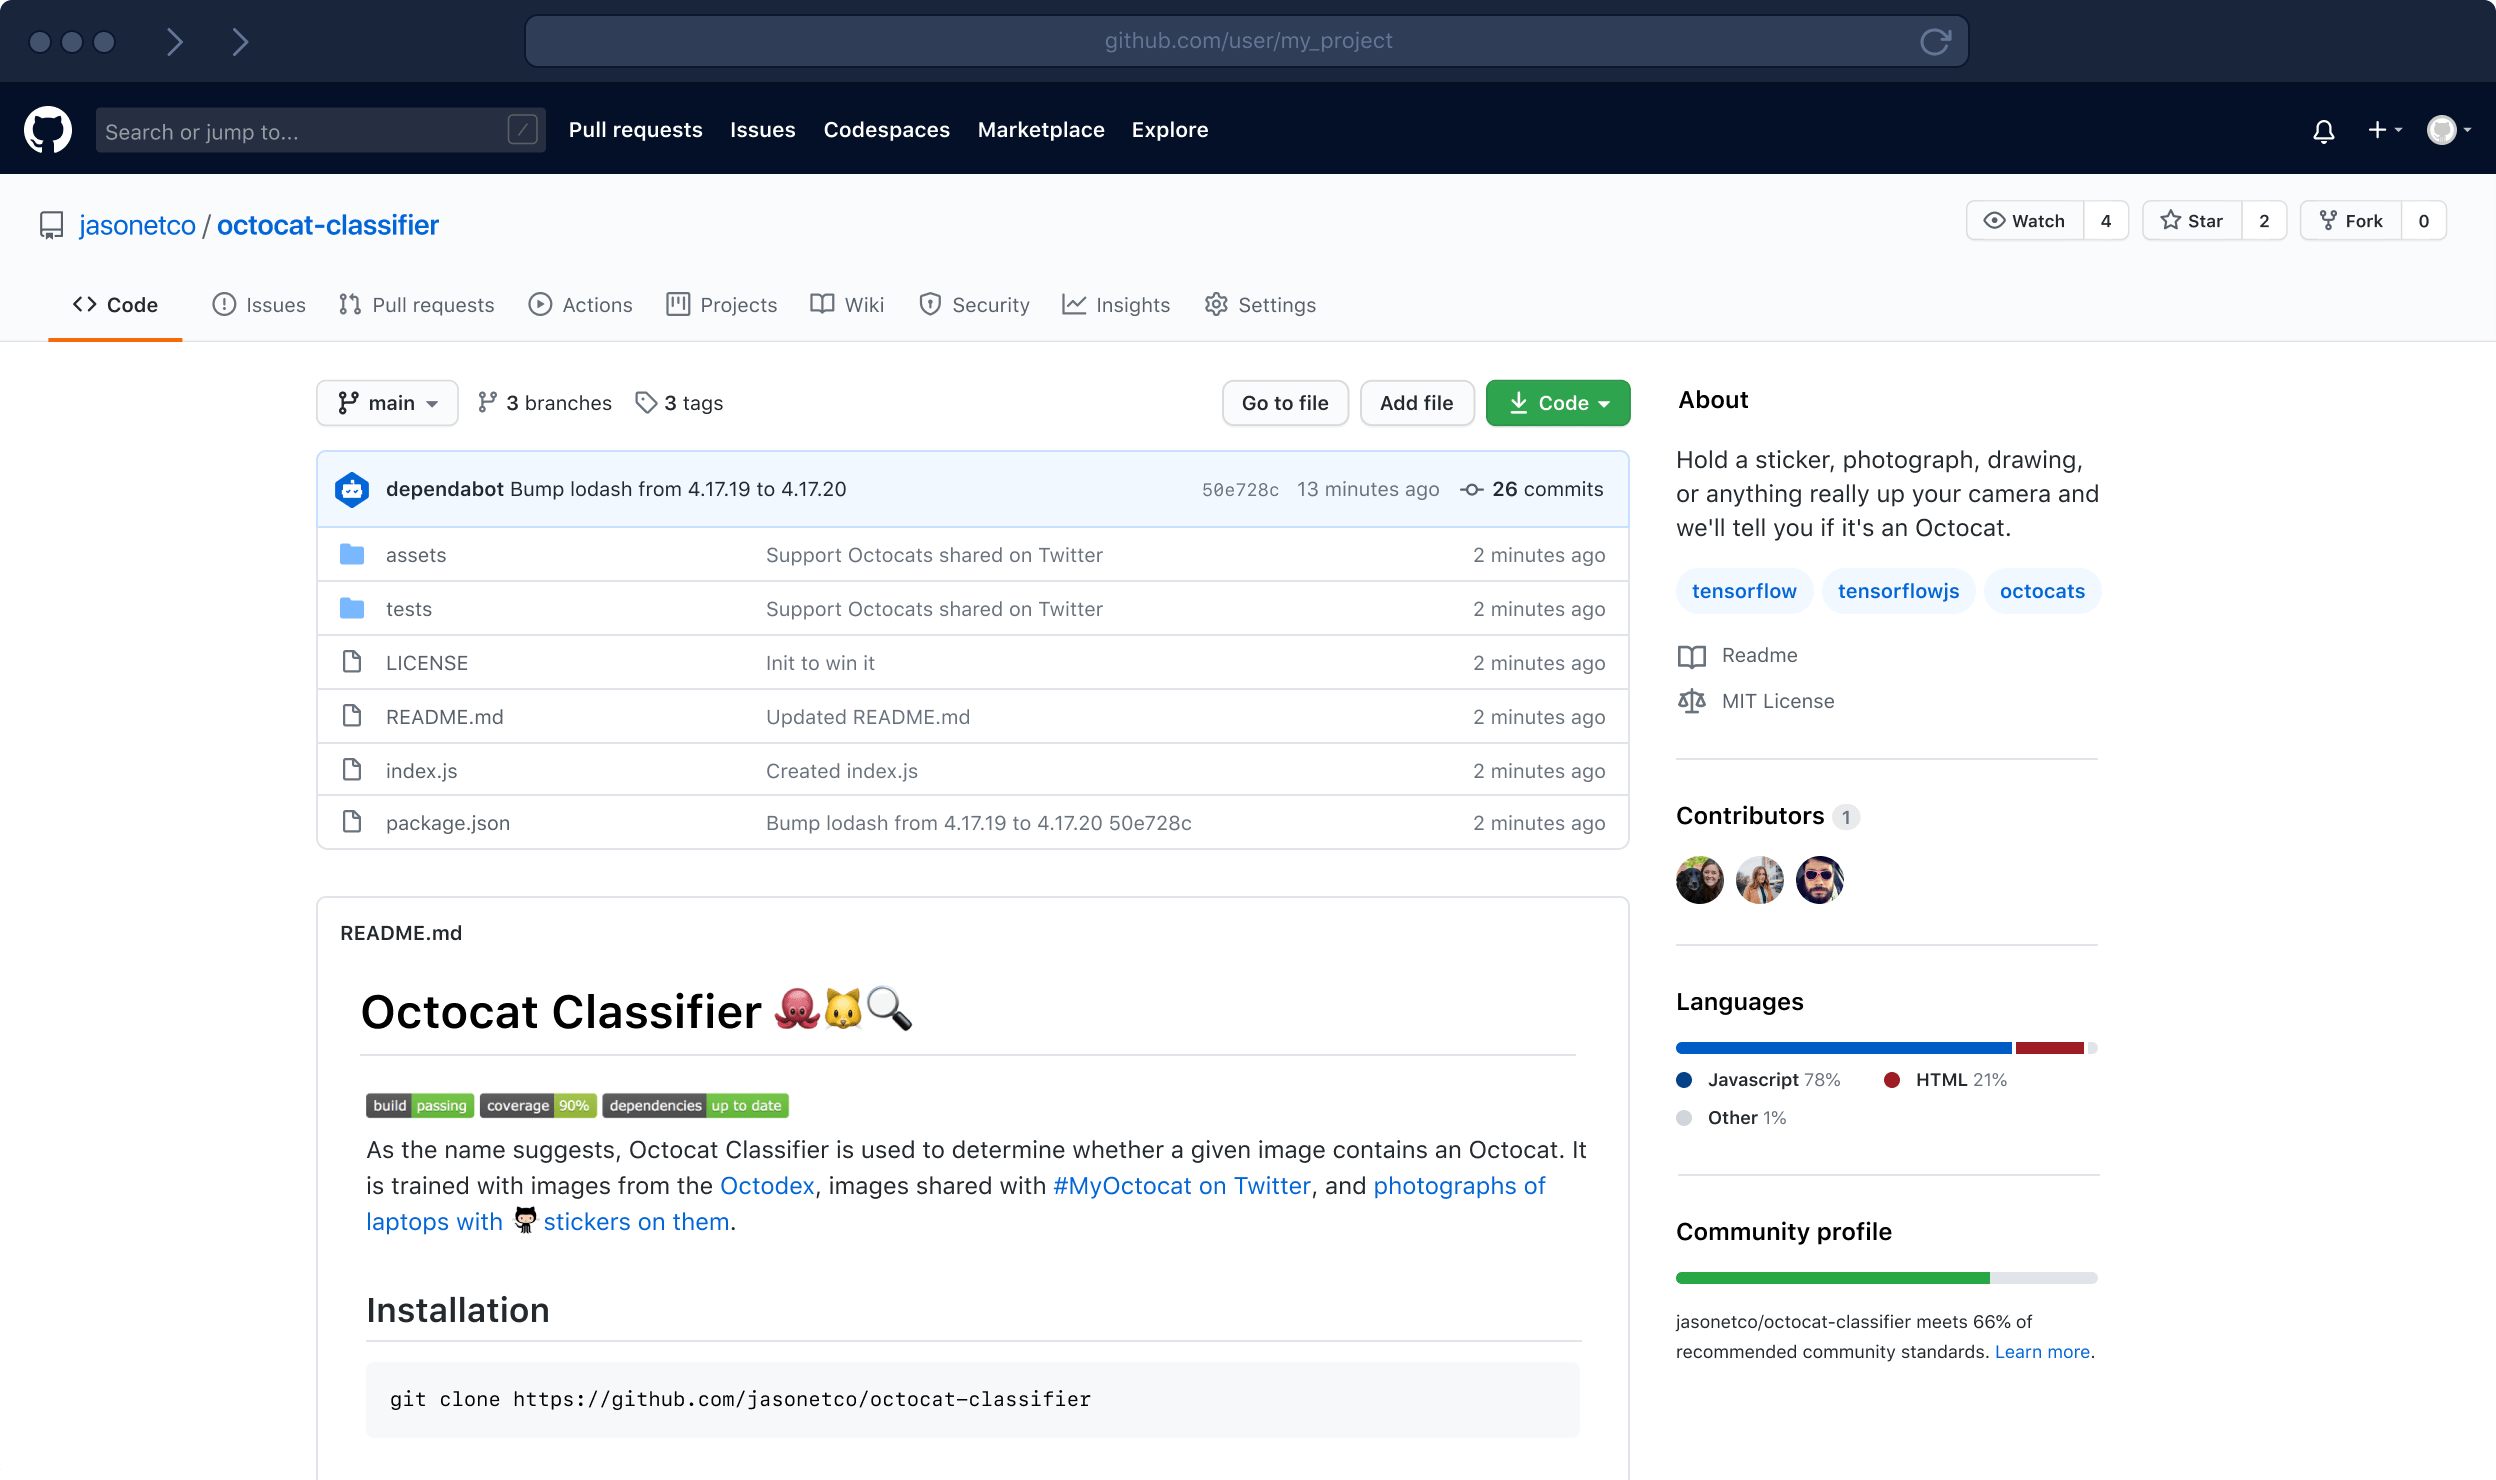
\includegraphics[scale=0.15]{img/githubpic.png}
  \centering
  \caption{Example of GitHub Repository}
  \label{fig: GitHub Repo Example}
\end{figure}
The GitHub repository where this project is located in contains two specific folder, my 'meal-planning' folder which contains the main application of the project (including the front end and back end of my application) and the 'img' folder which contains images used in my application. \\ \\
Apart from this folder my project also contains the files for the dissertation including the 'content.tex', 'project.tex', 'bibliography.bib', the project.tex which contains the cover sheet of the dissertation, content.tex which contains the chapters and sections written and the bibliography.bib which contains the primary, secondary and tertiary resources that are cited in the dissertation. \\ \\ 
There is a README.md file which contains information on why this repository exists, what is in it and how to run the project.  \\  \\
There is also a LICENSE.txt file which is used as a software license agreement. \\ \\
You can view the github by clicking the link as follows: \\  \\ \url{https://github.com/Emmanuel-Osabuehien/AppliedProjectMinorDissertation}

\chapter{Methodology}

\section{Overview}

In this chapter, I will give a quick overview on what is Methodology.\\ \\
During the process of creation my application, I research different approaches, testing and validation to keep my project organized. I adopted the Agile (incremental and iterative) approach for my project, I set up sprints where I set up tasks needed to be completed in a two week period. I also used Test Driven Development (Selenium and JUnit) where I wrote tests with enough code to allow it to pass without bugs, error and fault which I will later on edit this very same code.

\section{Agile Methodology}

In this section, I will discuss what is methodology, different types of methodology and how I implemented methodology in my project.

\subsection{What is Agile Methodology}

Agile is both an incremental and iterative approach to project management and software development that helps teams deliver value to their customers faster according to 'Atlassin', one of the leading examples of Agile framework. Scrum, DevOps, Trello and Jira are only a few examples. The Agile Manifesto outlines the principles that all Agile techniques follow. I'll be utilizing Trello for the duration of this project. Continuous improvement and incremental delivery are key to all Agile approaches.

\begin{figure}[H]
  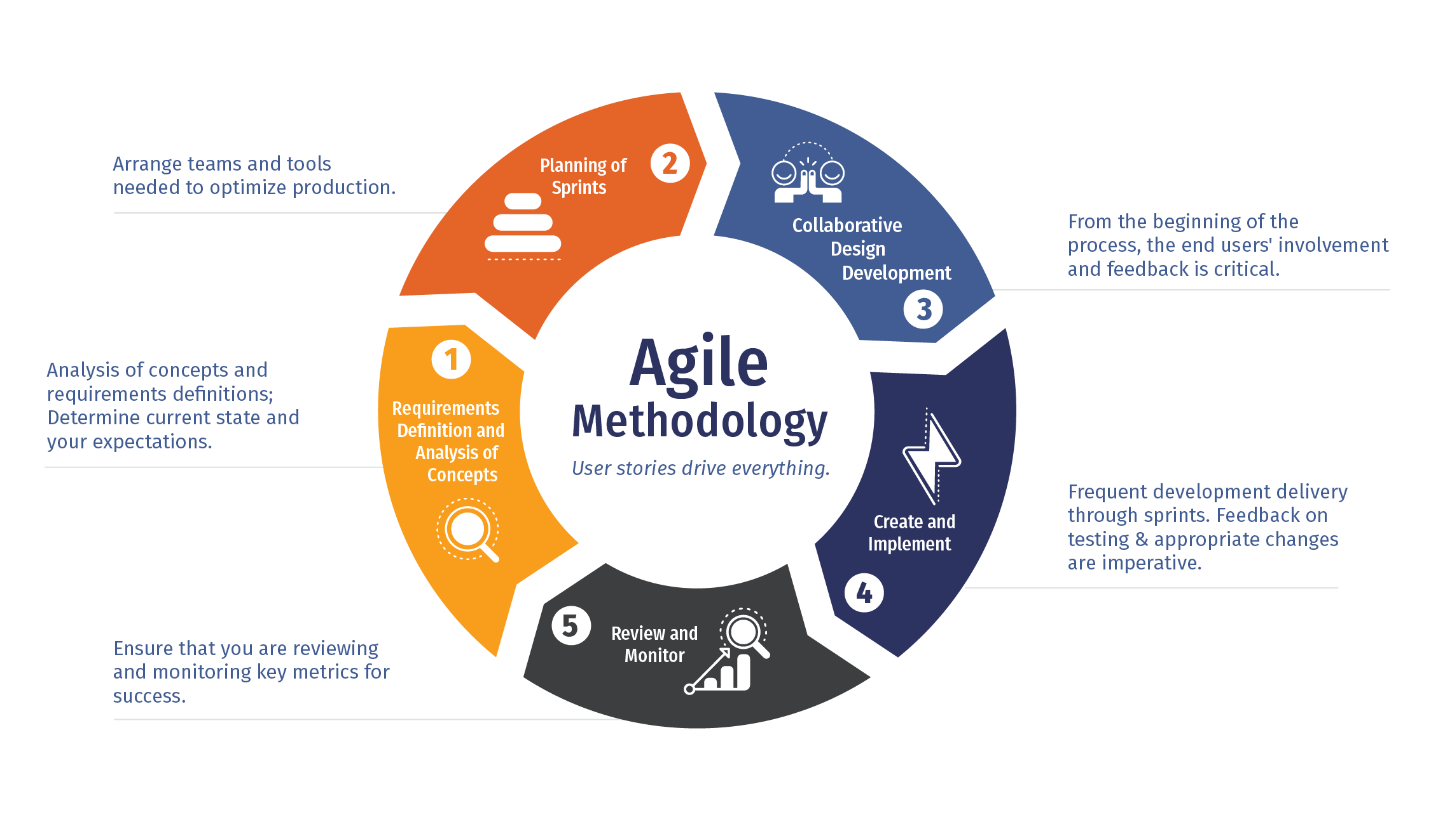
\includegraphics[width=\textwidth]{img/agilemeth.png}
  \caption{Agile Methodology}
  \label{fig: Agile Lifecycle}
\end{figure}

\subsection{Atlassian}

Q. Why did I choose Atlassian as my Agile framework?\\ \\
\begin{wrapfigure}{r}{0.5\textwidth}
  \begin{center}
    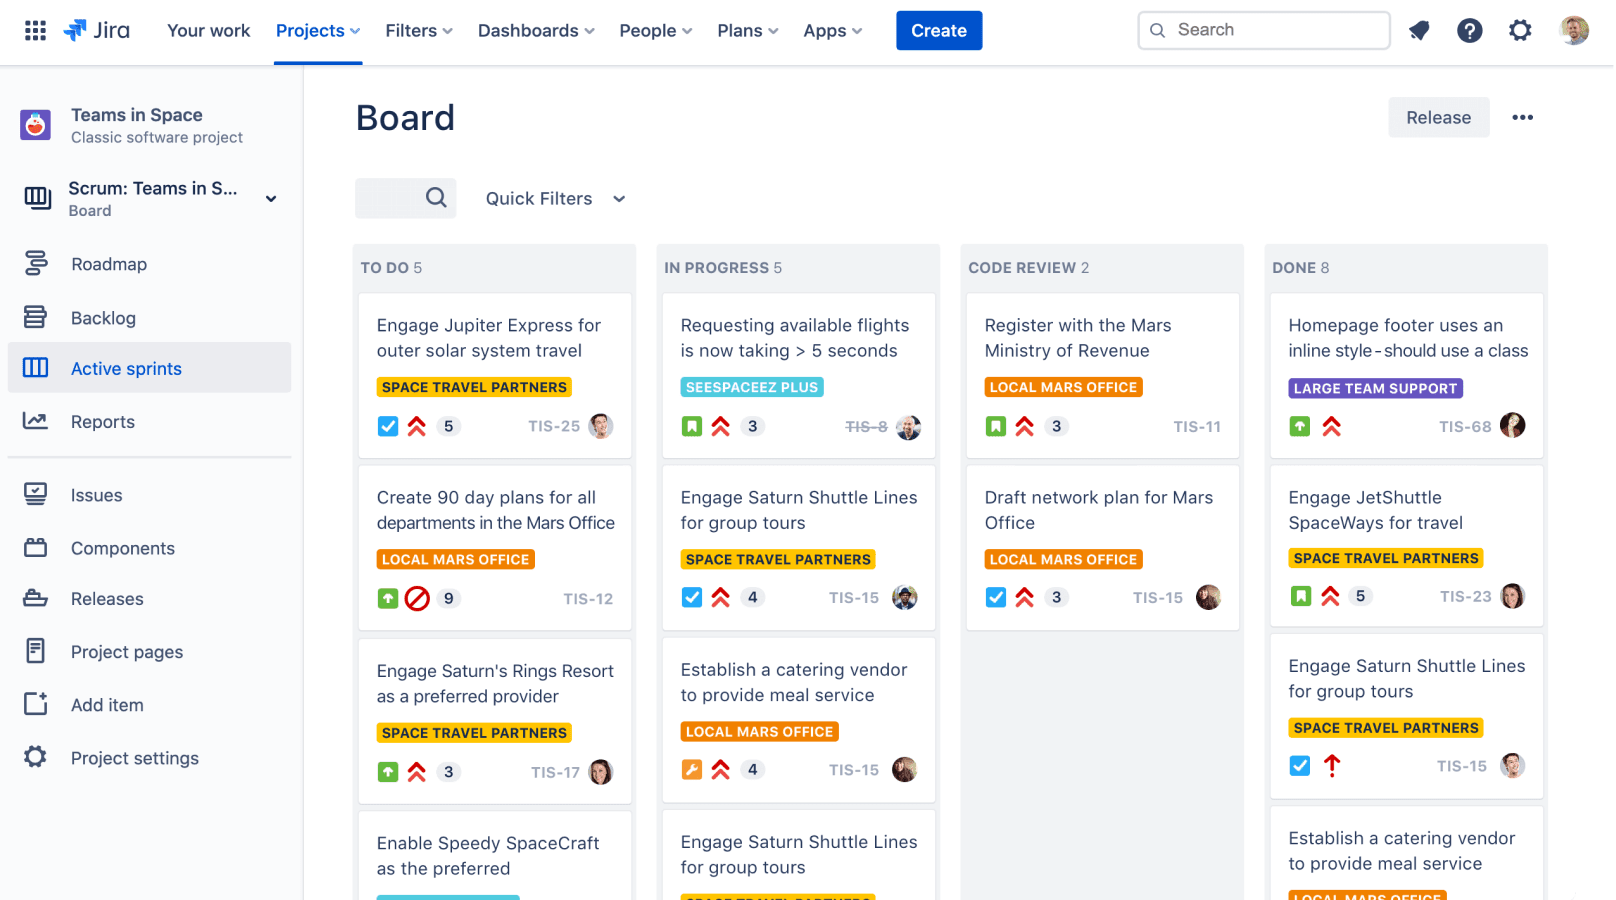
\includegraphics[width=0.75\textwidth]{img/atlasboard.png}
  \end{center}
  \caption{Atlassian Board}
  \label{fig:Example of Atlassian board}
\end{wrapfigure}
A. Atlassian gives the user (or a team) a clear view into the status, progress, and success of projects.  Also, they issue Power Ups to help you work across boards, with an visually appealing user interface.\\ \\
Atlassian also offers features such as:

\begin{itemize}
\item Following production workflow
\item Organizing future projects
\item Keeping track of project developmental process
\item Managing development schedule
\end{itemize}

\subsection{Implementation}

I implemented Trello with my project by connecting my GitHub repository to my project and I set up my sprints in my backlog and added tasks that were to be completed to my working board. I created 3 sections to my board for my working project known as "To Do", "Doing" and "Done", 'To Do' contained issues that were just added, 'Doing' contained issues that are in progress of being completed and 'Done' contained issues that were completed. This helps with the output, outcome and productivity of my project as I can visualize what I need to do and work on in a set schedule. I also have 2 other sections "Backlog" and "Issues", "Backlog" contains all functionality desired in the product and "Issues" contains any bugs, errors or fault in code that needs to be checked.

\section{Validation and Testing}

In this section, I will discuss validation and testing, what they are in terms of software development, different types of software that supply validation and testing and how I implemented testing in my project.

\subsection{Test Driven Development}

Test Driven Development (TDD) is software development approach in which test cases for each functionality are created and tested first and if the test fails then the new code is written in order to pass the test and making code simple and bug-free.

\subsection{Implementation}

I designed and wrote test cases whenever I developed a code to perform a specific functions for my application such as a 'Add a meal to your list' or 'Delete a meal that you have added to the list', after this test was performed I wrote a significant amount of code so the test should not fail and pass and continued to edit the code.

\subsection{End To End Testing}

End To End Testing is a type of software testing to that includes testing a product to check the behaviour of the product runs as intended. This type of methodology is used to recreate real user scenarios to test and validate the product basically aims to replicate real user scenarios so that the system can be validated for code merging and ethics.\\ \\
End To End Testing revolves around testing the application from start to finish during the software development life cycle and is completed running automated testing and manual testing tactics.\\ \\
This testing is applied to make sure that throughout the development of the product to ensure as the product evolves the behaviour of each sub-system works as expected.

\subsection{Unit.js}

Unit.js is just one of the testing frameworks I used to perform automated tests. Unit.js is a open-source framework, it is used to write and run repeatable automated tests. Unit.js is used to perform Java tests and is one of the leading examples of regression testing. This allowed me test the database functions to make sure when the code is run it works smoothly and also make sure certain outputs were correct such as 'Tallying the shopping list cost'.

\begin{figure}[H]
  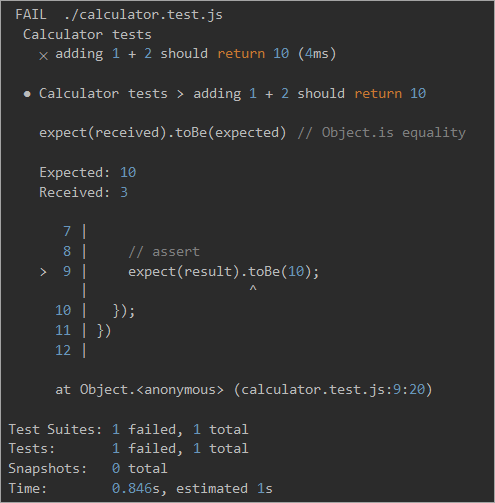
\includegraphics[width=0.77\textwidth]{img/unitjs.png}
  \centering
  \caption{Example of Unit.js Test Case}
  \label{fig: Unit.js Test Case}
\end{figure}

\subsection{Selenium}

I also used Selenium to perform automated tests for my application. 
Selenium is a open-source automated testing framework used to validate web applications across different browsers and platforms that can be used for multiple programming languages such as Java, JavaScript, Python, etc. 
Selenium is used to perform automation testing on such user interfaces and web pages, I implemented Selenium in my React application using Node and this allowed to test the database functions to make sure when the code is run it works smoothly.

\begin{figure}[H]
 \begin{center}
  
\includegraphics[scale=0.25]{img/seleniumlogo.png}
  \end{center}
  \caption{Selenium Logo}
  \label{fig: Image of Selenium Logo}
\end{figure}

\section{GitHub}

In this section, I will discuss the importance of GitHub during the development of my project. \\ \\
GitHub and Git were both very important in the development of my project. I used GitHub to manage all my files and folders regarding my project, repeatedly pushing these files/folders to GitHub whenever progress was made. I used GitHub with my Trello Boards where I would manage issues that arose during the development stages.\\ \\
\begin{wrapfigure}{r}{0.5\textwidth}
  \begin{center}
    
\includegraphics[width=0.35\textwidth]{img/githublogo.png}
  \end{center}
  \caption{GitHub Logo}
  \label{fig:Image of GitHub Logo}
\end{wrapfigure}
GitHub also allowed to me to use multiple branches where I created separate branches 'Main' and 'Master' where I would use Main for my finished code that had been tested and 'Master' for tested certain features which allowed me freedom to perform automated tests for debugging my application. \\ \\
GitHub also provides me with the option of return to previous iterations of my project, so in the case of an errors in the system I can just start again from a previous working and tested version as well as a page dedicated to issues where I can post issues that would then be divided into 2 week sprints.

\section{Issues Faced}

In this section, I will discuss the issues that I faced during the development of my project.

\subsection{Project Timeline}

The project timeline (or organization) was one of the issues I faced during the development of my project as dealing with a variety of different projects and trying to balance them all together was a difficult task that I had to solve. I solved this issue by creating a weekly schedule where I would allocate a select amount of time for different modules and project that I was working on so I didn't focus and stress about one project more than another.

\subsection{Underestimating The Scope}

The project scope was another issue I faced as I went through several ideas for my project and struggled with identifying if any of those ideas was the correct scope for my project. I overcame this obstacle by having weekly meetings with my supervisor where we would discuss on if the scope of my idea was right until coming to a conclusion.

\subsection{Feature Overload}

Feature overload was another issue that was faced during the development of my project as trying to select the right software/technology was difficult as I stressed how multiple types of software would gel together until I decided to use a MERN Stack that all flowed together smoothly and worked well together.

\chapter{Technology Review}

\section{Overview}

In this chapter, I will give a quick overview on different React/JavaScript libraries and frameworks, programming languages, programming software, and REST/Database Architecture that I used to develop my application.\\ \\
During the process of creation my application, I set up a list of features, components and functions that I wanted my application to fulfill by the time of completion. I would at times add to the list during the developmental process of my application. To complete this list, I would research the coding features, frameworks and libraries that would allow me to complete each task I set out for myself and attach each feature, framework or library to a task.

\section{MERN Stack}

In this section, I will discuss the technologies MongoDB, ExpressJS, ReactJS and NodeJS.

\subsection{MongoDB}

MongoDB is a cross-platform, document-oriented NoSQL database that uses collections and JSON type documents allowing databases to store high volume data storage, an alternative to most traditional relational databases such as MySQL that use table and rows. The addition of JSON allows data stored to be retrieved and updated. An example of retrieving data can be as follows, here is an example of document that can be modeled in MongoDB:
\begin{minted}{json}
{
  "user": {
    "email": "user1@example.com",
    "password": "password1"
  }
}
\end{minted}
If I can then run code to retrieve specific data that is stored, for example I can retrieve the above user's email as follows:
\begin{minted}{js}
user.email();
\end{minted}
Then once the code is run I should retrieve the user's email as follows:
\begin{minted}{json}
"email": "user1@example.com"
\end{minted}
MongoDB provides key feature such as scalability as you can run hundreds of nodes and millions of documents, replication providing many replica sets that can be used as a primary and secondary set at any time, indexing which improves the  the performance of searches in the database and MongoDB can be run across multiple servers. MongoDB is used by applications such as Uber, Forbes and Lyft.
\subsection{ExpressJS}

ExpressJS is an open-source, server-side web application framework utilized in building and designing either single-page, multi-page or hybrid web applications. There is many advantages to ExpressJS such as it works at a fast work rate, it is easy to learn, it provides predetermined code for developers to use and only knowledge of JavaScript and HTML is necessary. ExpressJS allowed me to utilize it's use of routers to add, edit and delete data to and from our database. \\ \\
Since I decided to use NodeJS instead of Yern, it only made sense to use ExpressJS due to how well they work together. ExpressJS provides middleware that is responsible for making decisions to give the correct responses for the requests made by the client. Express allows us to get and push data in a JSON format which will then have later use and he use of the routers helped me with four key features that I implemented in my app, these features were registration, logging in, adding/deleting meals from list and designing personal shopping lists. \\ \\
A quick example using ExpressJS to set up a simple request handler can be viewed below:
\begin{minted}{JavaScript}
'use strict'

var express = require('../../');

var app = module.exports = express()

app.get('/', function(req, res){
  res.send('Hello World');
});

/* istanbul ignore next */
if (!module.parent) {
  app.listen(3000);
  console.log('Express started on port 3000');
}
\end{minted}

ExpressJS was great in setting up the back end of my application as it allowed me to perform functionality such as adding data, updating data and removing data in our app.

\subsection{ReactJS}

ReactJS is an open-source, client-side JavaScript library used to build user interfaces especially for single-page applications as well as using reusable UI components (many of these components I will discuss in more detail). React was very useful as I was building a large scale web application where data was to be changed quite frequently especially without attempting to refresh the page, for example If I add a meal to my list it should be viewed instantly in the page or whenever a user has logged in our logged out they do so without the page reloading. React also provides many libraries which I will discuss later on that were very useful in creating my application such as Bcrypt which I used to encrypt any user password that was passed to the database. The addition of these libraries as well as my knwoledge of JavaScript and it's relationship with NodeJS and ExpressJS is why I chose ReactJS over software such as Angular which was highly considered.\\ \\
React provides many features such as JSX , UI Components:
 \begin{itemize}
  \item JSX - This is a JavaScript syntax extension.
  \item UI Components - This is necessary when mainting code for large scale projects.
  \item Flux - This helps keeping your data unidirectional.
\end{itemize}
A quick example of employing ReactJS can be seen below:

\begin{minted}{JavaScript}
ReactDOM.render(
<h1>Hello, world!</h1>,
document.getElementById('root')
);
\end{minted}

ReactJS provides many advantages for example, React can be used for both the front end and back end of you application, React uses DOM (Document Object Model) which improves apps performance and the use of components maintaining code improving large scale applications. ReactJS is used by applications such WhatsApp, Netflix and Atlassian.

\subsection{NodeJS}

NodeJS is an open-source, cross-platform, server-side run time environment. Node.js is asynchronous, event-driven enviornment designed to build scalable web applications. NodeJS is integral in handling multiple HTTP requests concurrently these request can be either a GET request, POST request. PUT request and DELETE request. NodeJS was very important in my application as it was needed to perform tasks such as adding users to our database and also adding meals and ingredients to each users documents.\\ \\
The NodeJS website (https://nodejs.org/) provides an example of setting up your run time environment, here if the enviornment is set up correctly, when the user enters https://localhost:3000/ into their browser the message "Server running at https://localhost:3000/ " will be printed in your console and the status code 200:
\begin{minted}{JavaScript}
const http = require('http');

const hostname = '127.0.0.1';
const port = 3000;

const server = http.createServer((req, res) => {
  res.statusCode = 200;
  res.setHeader('Content-Type', 'text/plain');
  res.end('Hello World');
});

server.listen(port, hostname, () => {
  console.log(`Server running at http://${hostname}:${port}/`);
});
\end{minted}
NodeJS contains many advantages such as the speed and performance, providing reusable code, it's ability to handle multiple requests and it's scalability.
NodeJS is used by applications such eBay, Linkedln and Yahoo.

\section{Languages}

In this section, I will discuss the programming languages I used to develop my project.

\subsection{JavaScript}

JavaScript is a high-level, text-based programming language that can be used for both the client and server side. JavaScript allows user to fully engage and interact with web pages as you can use it to calculate, manipulate and validate data and is typically assisted by HTML and CSS.\\ \\
JavaScript is was very useful for my app as JavaScript itself is highly influential in building web apps and web servers as well as developing the interactive behaviors of my web app such as retrieving the users meals data and checking the login details of a pre-existing user.\\ \\
An example of using JavaScript to calculate data can be shown below, where we see an example of a user entering two input values that will be added together:
\begin{minted}{JavaScript}
const num1 = 5;
const num2 = 3;

// add two numbers
const sum = num1 + num2;

// display the sum
console.log('The sum of ' + num1 + ' and ' + num2 + ' is: ' + sum);
\end{minted}

\subsection{HTML}

Hyper Text Markup Language also known as HTML, is a standard markup language used to create, design and structure web pages and also consists of a series of elements, it is typically assisted with the programming languages JavaScript and CSS.\\ \\
A quick example of a HTML document is shown below:

\begin{minted}{HTML}
<!DOCTYPE html>
<html>
<head>
<title>Page Title</title>
</head>
<body>

<h1>My First Heading</h1>
<p>My first paragraph.</p>

</body>
</html>
\end{minted}

\subsection{CSS}

Cascading Style Sheets also known as CSS is a style sheet language that controls the layout of web pages and it is used to describe how HTML elements are to be displayed on screen.\\ \\
Here is an example of code from my meal planning app that I used to design the body of one of the pages:

\begin{minted}{CSS}
body {
    padding: 0px;
    margin: 0px;
    background: #F4F1F1;
    font-family: 'Open Sans', sans-serif;
    color:black;
    font-size: 15px;
}
\end{minted}

\section{JavaScript Frameworks}

In this section, I will go through the frameworks provided by JavaScript that I used to develop my project.

\subsection{Axios}

Axios is a promise-based HTTP Client for node.js and the browser. Axios is what I used to send requests and retrieve responses using the client-server model. Axios played a huge role in my application as it was very necessary in completing the functionality of reading, adding, editing and deleting from my database. I considered using the fetch method instead of using Axios but after deliberating  and researching differences between the two, Axios has the advantage of being better at error handling.

\subsection{CORS}

Cross-Origin Resource Sharing also known as CORS, is a mechanism that allows or prevents requested resources on a server depending on where the request was initiated. I used CORS in my app to load in the API and all the data involved in the API that I used for my project (TheMealDB API), it was an easy decision to choose to use CORS as it was a JavaScript library that I found easy to understand and use.

\subsection{Nodemon}

Nodemon is a command-line interface utility that develops node.js based applications by watching the file system and automatically restarting the node application when a file change has occurred and is detected. I found Nodemon great to use instead of many alternatives due to Nodemon not requiring any additional changes to your code or method of development. Nodemon was simply used as a way to not have to continuously restart my application to make the added changes to my app instead Nodemon will just rerun the app and make the added changes as intended.

\section{JavaScript Libraries}

In this section, I will go through the libraries provided by JavaScript that I used to develop my project.

\subsection{Bcrypt}

Bcrypt is a password-hashing function used to convert a string of input data to a fixed, unpredictable output. I used Bcrypt to encrypt the password of all registered users to enhance user security, so when a user registers into the system with an email and password, the password will be automatically encrypted.

\subsection{Bootstrap}

Bootstrap is a free, open-source toolkit used to create web pages and applications on the applications front end using HTML, CSS and JavaScript templates such as forms, buttons, jumbotrons, etc. I used Bootstrap to design the majority of the web pages for my application using the aforementioned templates that come with Bootstrap.

\subsection{Chart.js}

Chart.js is an open-source, JavaScript library that is used for visualizing data, that allows designers and developers to draw all kinds of charts using the HTML5 canvas element.\\ \\
This includes 8 different charts:

\begin{itemize}
    \item Line Chart
    \item Pie/Doughnut Chart
    \item Bubble Chart
    \item Bar Chart
    \item Radar Chart
    \item Polar Chart
    \item Area Chart
    \item Scatter Chart
\end{itemize}

I used Chart.js to develop a web page that contains a table full of charts that contain different diets that users can follow and read about as each chart contains a hyperlink to a web page giving more insight about a specific diet.

\subsection{JsonWebToken}

JsonWebToken is an open standard used to share security information between the client and a server. I used JsonWebToken to generate Tokens that users can use to log in to their accounts for increased security as opposed to just entering email and password.

\subsection{Mongoose}

Mongoose is a JavaScript library that creates a connection between MongoDB and the Express web application framework. As previously mentioned, I used Mongoose as my way to connect my database to my web application.

\section{React Component Libraries}

In this section, I will go through the libraries provided by React that I used to develop my project.\\ \\

\subsection{Create-React-App}

Create-React-App is a comfortable environment for learning React, in my opinion it is the easiest way to start building a new single-page or multi-page application in React. Create-React-App will automatically set up the coding environment to use JavaScript features. I used Create-React-App to set up my enviorment for my application. 

\subsection{React-Bootstrap}

React-Bootstrap is a front end, component-based library that provides native Bootstrap components as pure React components such as buttons, modals, cards, etc. I used React-Bootstrap as it converts JavaScript to React aimlessly.

\subsection{React-Router}

React-Router is a standard library for routing in React. It enables the navigation of various components in a React Application, allows redirecting the URL of the browser, and keeps the user interface in sync with the URL. I used React-Router to develop and define my routes for my application and connect it to my navigation bar that I implemented into my app.

\subsection{React-Router-Dom}

React-Router-Dom is an node.js package that enables you to implement dynamic routing in a web app. It allows you to display pages and allow users to navigate them. It is a fully-featured client and server-side routing library for React. Look at the above section about 'React-Router' to view why I decided to use React-Router-Dom as the reason is exactly similar to the aforementioned section.

\section{Architectural Styles and Patterns}

In this section, I will discuss the architectural styles or patterns, going through what they are, why they are necessary and the principles to be followed.

\subsection{REST}

Representational State Transfer also known as REST is an architectural style or pattern used to obtain a standard between operating systems allowing communication to be improved upon.\\ \\
Not unlike many other architectural styles, REST has a list of guiding principles that need to be pleased and obtained.\\ \\
These non-negotiable guideline principles are as follow:

\begin{itemize}
    \item \textbf{Uniform Interface:} This is a key constraint which defines the interface between clients and servers. It simplifies and decouples the architecture, which enables each part to evolve independently. The following four constraints:
    \begin{itemize}
        \item \textbf{Resource-Based:} In the interface, individual resources are identified in requests. An example can be to log in as a specific user that has been registered on the site:
        \item \textbf{Resource Representation:} The resources should have uniform representations in the server response. Client has representation of resource and contains information to modify or delete the resources on the server. This representation can be in HTML, XML, JSON, etc.
        \item \textbf{Self-descriptive Messages:} Each resource includes information to describe how to process the message so that server can analyses the request.
        \item \textbf{Hypermedia as the Engine of Application State:} The client should have only the initial URI of the application. It also needs to include hyperlinks for every response so that the client can discover other resources.
    \end{itemize}
    \item \textbf{Client-Server:} The client send a request and the server sends a response executing the concerns to stay separate which in turn helps the components stay independent.
    \item \textbf{Stateless:} A client can send multiple requests where each are independent carrying enough information necessary to understand and process. The server is not able to information that has already been stored in the server. 
    \item \textbf{Cacheable:} The cacheable constraint requires that a response is either cacheable or not. The client cache is only given the right to reuse that response if it is cacheable.
    \item \textbf{Layered System:} The layered system allows the architecture to be composed multiple layers. Each individual layer has no clue of other layers with an exception to the immediate layer that they are engaged with.
    \item \textbf{Code On Demand:} This is an optional feature which allows client functionality to extend by downloading and executing code in the form of scripts. The reducing of the number of features needed to be pre-determined simplifies the downloaded code. Servers can also provide executable code to the client.
\end{itemize}

Here is a example of a REST Model:

\begin{minted}{js}
{     
    "firstName": "Ryan"
    "surName" : "Holland",
    "age" : 22
}
\end{minted}

\section{API}

In this section, I will discuss the API(s) that I found and used in the development of my project.

\subsection{TheMealDB API}

For my project, I used a free to use API I found while searching online, it is called the TheMealDB API, this API contains a pre-determined list of recipes, there are many features that come with this API such as searching for meal by name, listing all meals by first letter and search meal details by id. The API also contains features that I didn't use but I found interesting to play around with such as looking up a single random meal, looking up a selection of 10 random meals, filtering by main ingredients and listing all categories, area, ingredients.

\section{Databases}

In this section, I will discuss the use of databases and how it was implemented in my project.

\subsection{MongoDB Atlas}

For my project, I used the MongoDB Atlas this is a free, multi-cloud database service that is dedicated to consistent performance, advanced security and unlimited scalability, this was designed by the same people who built MongoDB. MongoDB Atlas allows users to deploy and manage databases while building global applications on the cloud. I chose to use the MongoDB Atlas due to the connection with MongoDB in addition to it is cost-effective, it can be easily accessed by the web server and various schemas can be constructed. App users can access the database by registering and entering their user details.

\section{Validation and Testing}

In this section, I will discuss the validation and testing that was conduced during various phases of my project development.

\subsection{Unit.js}

Unit.js is a JavaScript testing framework that is a method for end to end testing. An open-source framework, it is used to write and run repeatable automated tests. End-to-end testing is a technique that tests the entire software product from beginning to end to ensure the application flow behaves as expected. Unit.js testing was necessary when testing if any new changes to code or added features to my project. I considered other frameworks such as WebdriverJS and NightwatchJS but there were many benefits of Unit.js such as the improved code quality, early fault/error discovery and generating code reports.

\subsection{Selenium}

Selenium is a open-source, automated testing framework used to validate web applications across different browsers and platforms. Selenium has the advantage of being an add-on for most web browsers and also can test various different languages such as JavaScript, Python, Ruby, etc. Selenium keeps track of functionality, actions and changes that occur during each testing process of the application. Each test can then afterwards be reviewed. I had past experience using Selenium and it was a great addition to use during the development of my application as I would not have to manually test my project, this would help me finish all my objectives in a quicker time.

\section{Development Software}

In this section, I will discuss the different apps used to create my web application such as apps necessary for writing code, apps needed to upload files to a secure repository, etc.

\subsection{Visual Studio Code}

Visual Studio Code is a free, source-code text editor (IDE), the software is very lightweight but includes many features. It includes many powerful features such as refactoring, debugging, syntax highlighting, snippets, etc. A wide variety of languages can be used such as Python. C++, JavaScript, HTML, etc. I used Visual Studio Code to develop all my source code for my application and was the app I used to develop the front end of my project,

\subsection{Atom}

Atom is also is a free, source-code text editor (IDE), the big difference between Atom and Visual Studio Code is Atom is hackable. Features of Atom include highlighting, syntax checking, auto-completion, etc. Just like Visual Studio Code, Atom can support a wide variety of of languages such as Ruby, JavaScript, Python, etc. I used to develop the paths and back end of my application.

\subsection{Postman}

Postman is an API platform used to build and interact with APIs. It is a HTTP client test various HTTP requests such as GET, POST and DELETE and we then retrieve the response. I used Postman to test my functions and paths for my app to send requests to the server and retrieve the information.

\subsection{Git}

Git is a free, open-source distributed version control system that is used to deal with a scope of small to large projects easily. I used Git to track any changes in the set of files.

\section{Dissertation}

In this section, I will discuss the software I used to make up my dissertation accompanying my application.

\subsection{\LaTeX}

\LaTeX is a high-quality, software system for document preparation which is used writing documentation. \LaTeX was introduced back in the 1980's and is now considered the gold standard for creating scientific documentation. \\ \\
This academic year has been the very first time I have used \LaTeX and I have enjoyed using it very much and have used it any time documentation is needed for all of my modules.\\ \\
I was given a choice between using \LaTeX and Microsoft Word was due to many reasons, the popularity being one as was previously mentioned it has become the standard for documentation, the high quality being another reason and my final reason being the many packages that come with \LaTeX that you can use that I find very useful.

\subsection{BibTeX}

BibTeX is reference management software for formatting lists of references, this tool is typically used together with \LaTeX.\\ \\
Just like \LaTeX, this was my first academic year using BibTex and just like \LaTeX I enjoyed using BibTex and have used any time I am curating a document where I need to use references.\\ \\
The reason I used BibTex was mainly due to the different styling I can use to format my references.

\chapter{System Design}

\section{Overview}

In this chapter, I will give a quick overview on the front end, back end, database and REST architecture if my application, as well as the application features and functions.\\ \\
During the process of creation my application, as previously mentioned in the 'Technology Review' chapter, I set out a list of features, components and functions before I started the coding process of my application that I wanted my application to fulfill by the time of completion, which sometimes I added to during the developmental process of my application.\\ \\
Here we look at the design process of both the front end and back end architecture of the application as well as looking at how it may differ from standard meal planning applications.\\ \\
This app is a single-page application opposed to a multi-page application, I choose to use a single-page application because:

\begin{itemize}
    \item Easier debugging
    \item User Experience
    \item Less complex implementation
    \item Better caching
\end{itemize}

The client side is written in JavaScript, HTML and CSS as all these languages give the application an appealing universal appearance.\\ \\
The server side is written in NodeJS and ExpressJS as these provide libraries and frameworks which allow us to use a variety of attributes and features.

\section{Client Side}

In this section, I will discuss the components regarding the front end of my web application.

\subsection{Home}

When the application is first deployed the user is brought straight to home (dashboard). The page contains a number of the components that we are going to discuss later in more detail such as the Meal Listing, the Search Bar and the Jumbotron. This page is also what we use to set the standard for our user interface to give an idea into what is going to be the design for app and whether this design is good enough to give the app a universal look. Similar to all the other pages, the home page also contains the navigation bar which we will use to navigate across all the accompanied pages. The Home page is also the only page that is provided for both registered and unregistered users.

\subsection{Register}

When the register component is selected, if a user wants to progress further in the application to use any of the other components or features then the user must register in our application, they will only need to provide an email and password for a successful registration. Once a user complete the registration process and the user has logged into the application then can proceed and use all the features that the application provides including adding and removing recipes from a listing page. using the BMR/calories needed calculator, forming a personal ingredients list and researching various diets provided by the application. The registration component consists of a clear white background featuring two form boxes to enter your email and password and a sign up button. If a user enters an incorrect email format they can register and are asked to submit an official email with the proper format.

\begin{center}
  \begin{figure}[H]
    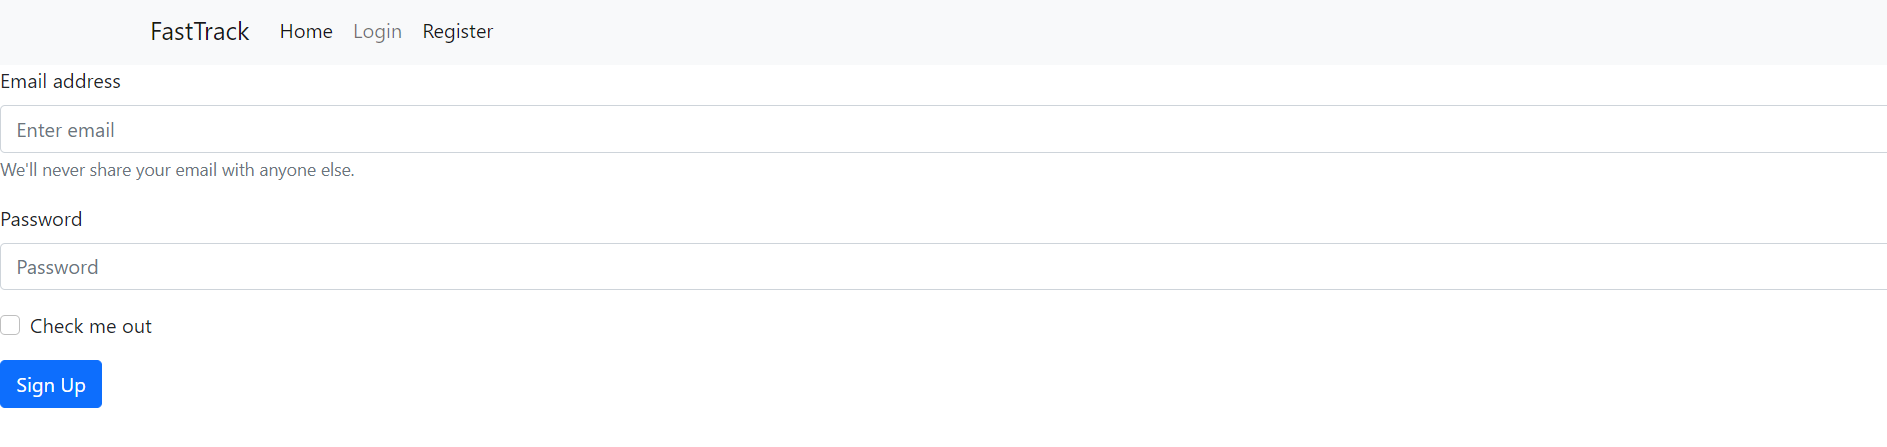
\includegraphics[width=\textwidth]{img/signup.png}
    \caption{Register Page}
    \label{fig: Image of Registration Page}
  \end{figure}
\end{center}

\subsection{Login}

As discussed in the 'Register' section, if a user want to use all the components and features that the application provides then they have to register and log in with a provided email and password. The component is a simple login page with a clear white background featuring two form boxes to enter your email and password and a log in button to process your credentials similar to the registration format, if the credential are correct then they are automatically logged in and have access to all components in the application but if the credentials are invalid they are sent an error message and are encouraged to enter correct details.

\begin{center}
  \begin{figure}[H]
    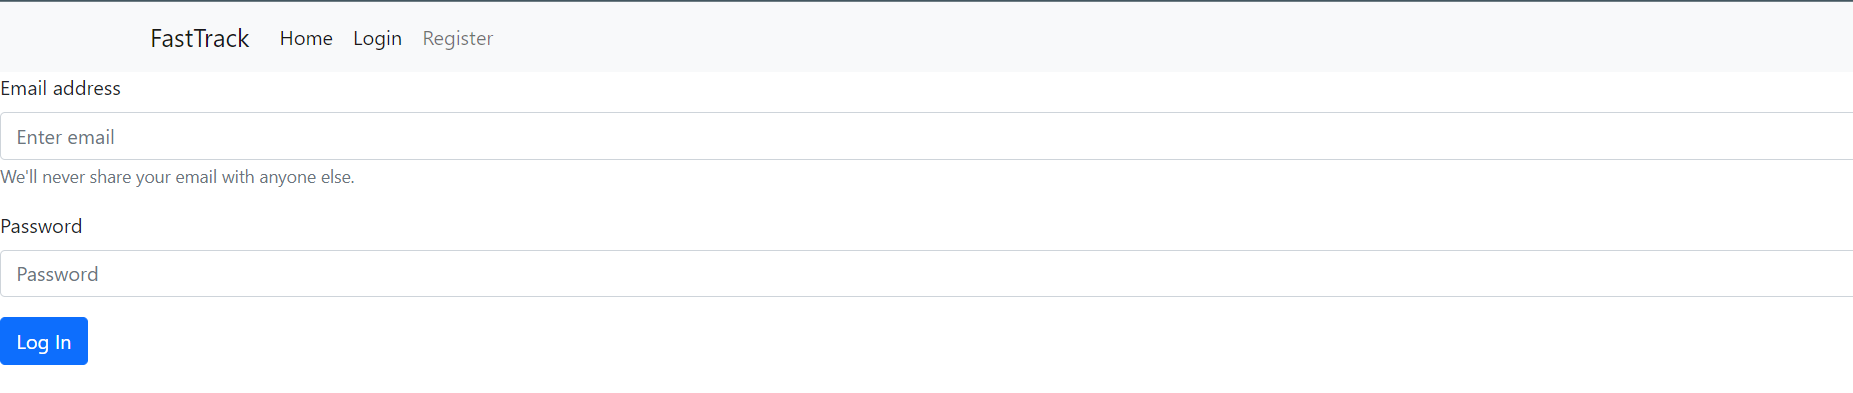
\includegraphics[width=\textwidth]{img/login.png}
    \caption{Login Page}
    \label{fig: Image of Login Page}
  \end{figure}
\end{center}

\subsection{Meal Landing}

The Meal Landing component consists of a list of meals (recipes) that has been pulled from the API that I used (TheMealDB API) and after the data has been fetched, the meals are then displayed and formatted in a HTML modal and card format to enhance the user interface of the app. On the card, the title of the meal, the id and the cooking method, when users can interact with the cards by clicking the 'See More' button on the card which where you are given two buttons, the first button is to exit this card viewing and the second is to add this selected meal to a meal listing page where you can view in more detail. Once you select the button to add the meal to the listing, straightaway the button is changed to remove the meal from the listing which when you click the meal is then removed from that same listing page, when you navigate to the meal listing component you can view all the meals that you have added. The meal landing page also changes when you use the search functionality in the dashboard component, when you type and search for a specific word, only the meals with a title that matches will appear in the landing component.

\subsection{Meal Listing}

The Meal Listing component is connected to the CRUD functionality of the meal landing component as the meal landing components allows users to add and remove (recipes) to the meal listing component, when a meal is added to the meal listing component, the meal is displayed in the exact same format as it is displayed in the meal landing component using the HTML card, modal and button and users can also add and remove meals from the meal listing as well. The meals added to this component are stored in the database document for the registered user and when it is removed it will be deleted from the database document.

\begin{center}
  \begin{figure}[H]
    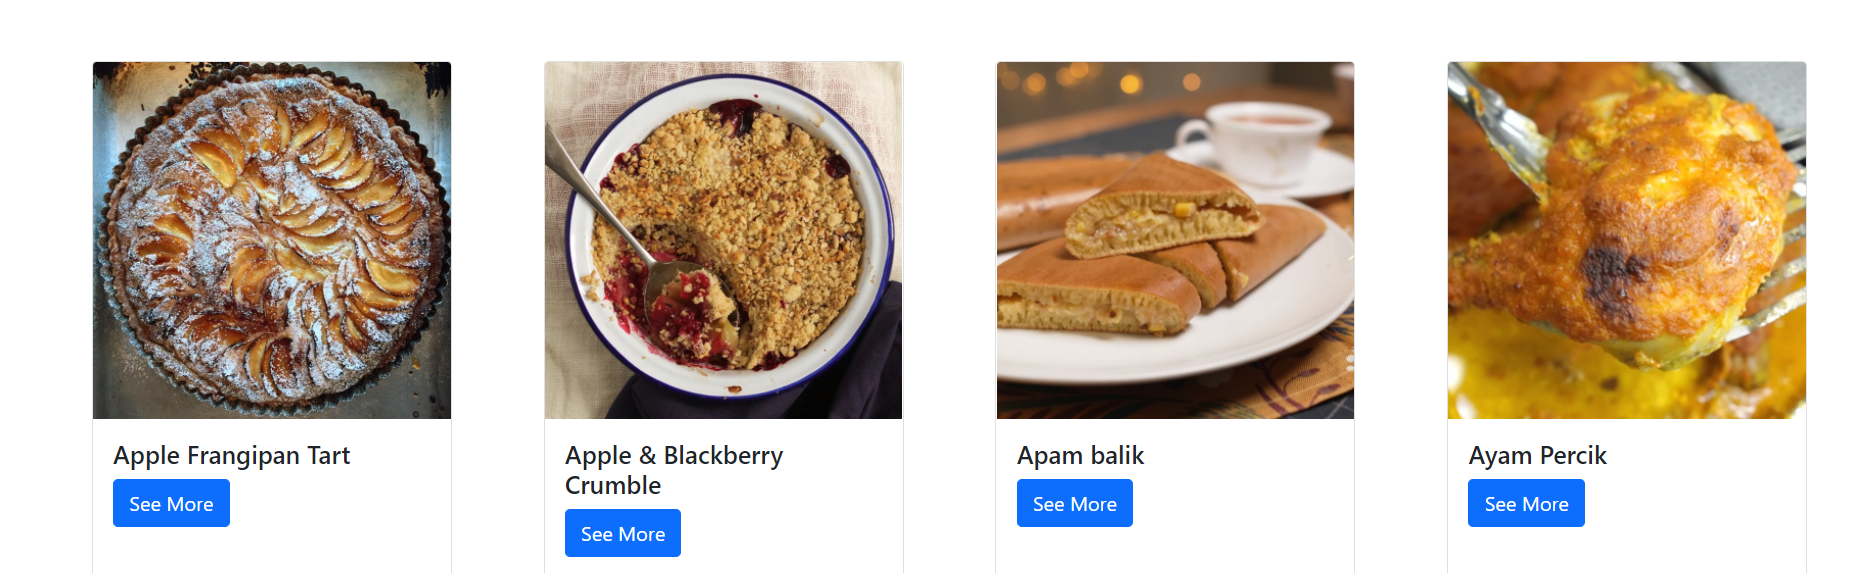
\includegraphics[width=\textwidth]{img/meallist.png}
    \caption{Mean Listing Page}
    \label{fig: Image of Meal Listing Page}
  \end{figure}
\end{center}

\subsection{Calories Calculator}

The Calories Calculator component is a calculator where users can calculate either their BMR (Basic Metabolic Rate) and the amount of calories the users needed based on the users details. When the user enters the page containing the component, the page consists of solely the calculator and when the users views and wished to use the calculator they must enter in specific details that calculator used to calculate the metabolic rate and calories needed, these details include the users age, gender, weight (in pounds), height (feet and inches) and their activity level. When all these details are entered the user is presented with two separate buttons, one button to 'Calculate BMR' which takes in the details entered and calculates the basic metabolic rate of the user based on these details and the other button to 'Calculate Calories Needed' takes in the details entered and calculated the amount of calories the users needs to consume in a day based on these details.

\begin{center}
  \begin{figure}[H]
    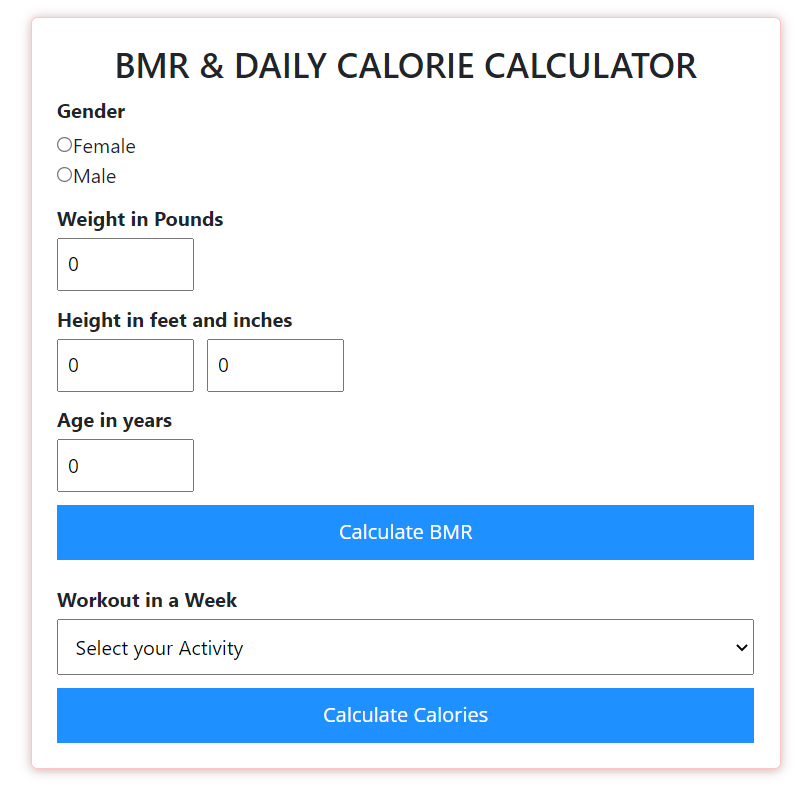
\includegraphics[width=\textwidth]{img/bmrcalc.png}
    \caption{Calories Calculator}
    \label{fig: Image of Calories Calculator}
  \end{figure}
\end{center}

\subsection{Shopping List}

The Shopping List component is a page where users can sort out a shopping list for themselves. It consists of a react table where users can organize their personal shopping/ingredients list where the user can view for later use. The shopping list is divided into two columns 'item name' and quantity, when the user adds an item it is then added to a total that adds up the quantity of items added to the list and is printed to the bottom of the table. After an item is collected the user can actually cross that item off the list by clicking a checkbox that sits beside each item on the list.

\begin{center}
  \begin{figure}[H]
    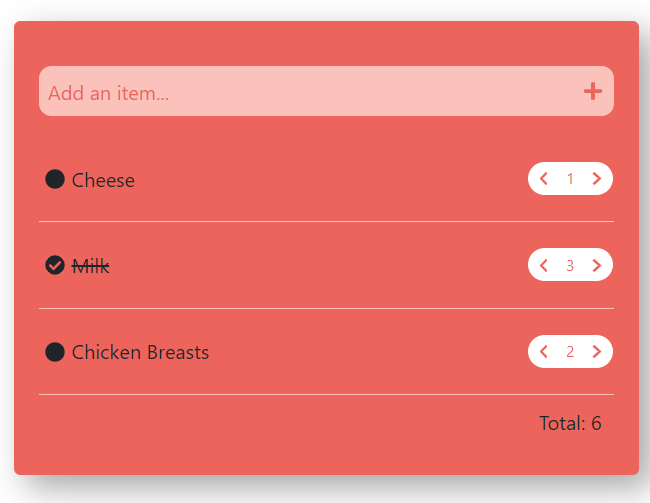
\includegraphics[width=\textwidth]{img/shoplist.png}
    \caption{Shopping List Page}
    \label{fig: Image of Shopping List Page}
  \end{figure}
\end{center}

\subsection{Dietary Requirements}

The Dietary Requirements component is a page of the application where users can research various dietary information of diets that the application provides. The page consists of a HTML table that contains various diet plans, for example a vegetarian diet, ketogenic diet and paleo diet. Each table consists of pie chart containing the percentage of protein, fats, carbohydrates and fruits/vegetables the user must follow for this specific diet as well as a hyperlink where user can gain more information of every diet.

\begin{center}
  \begin{figure}[H]
    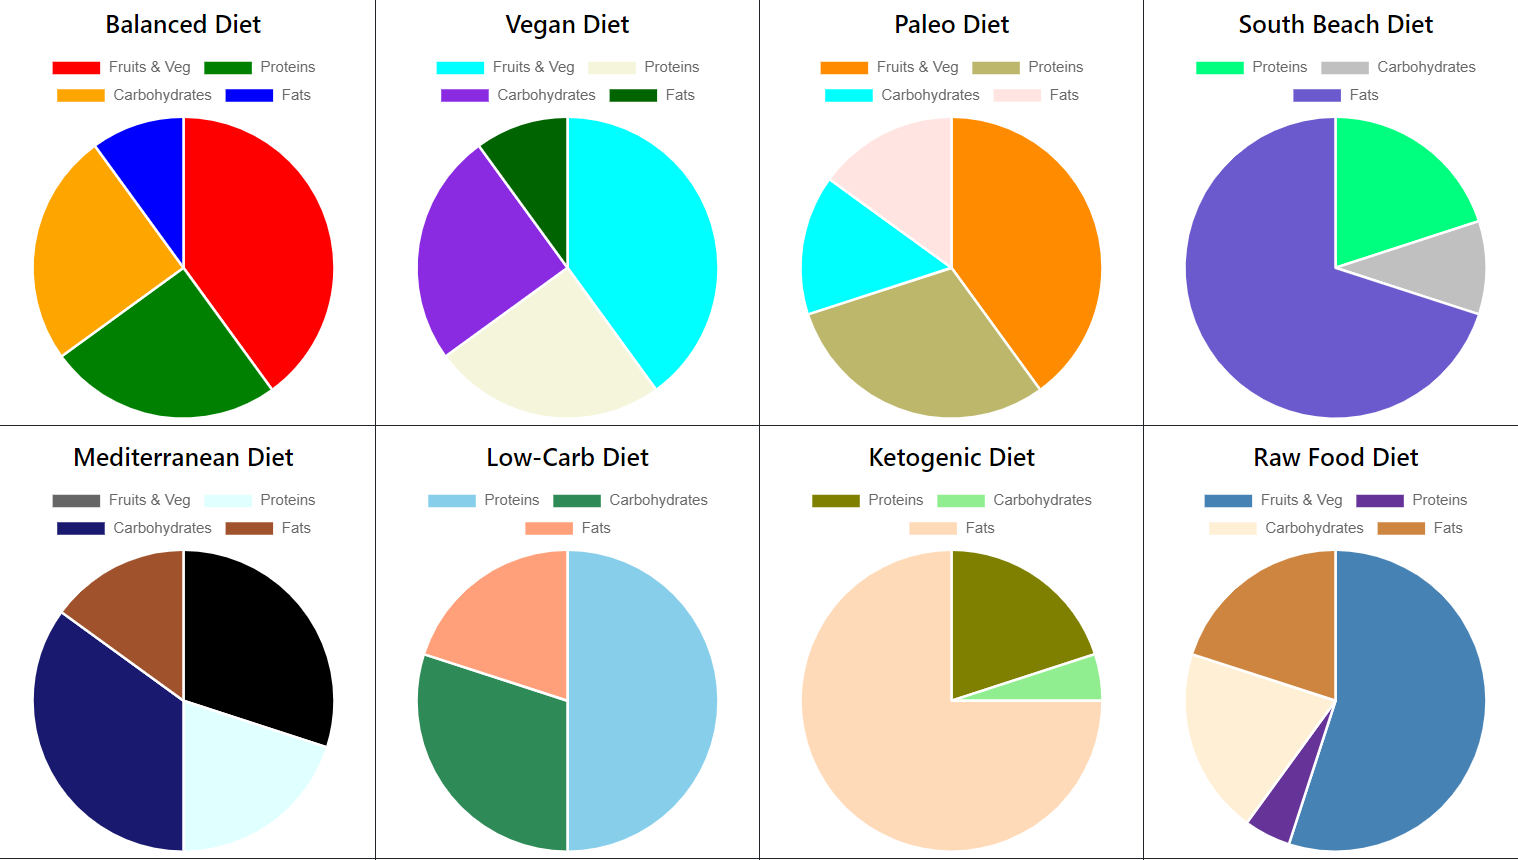
\includegraphics[width=\textwidth]{img/charts.png}
    \caption{Pie Charts}
    \label{fig: Image of Dietary Charts}
  \end{figure}
\end{center}

\subsection{Navigation Bar}

The Navigation Bar component is at the top of each page as you navigate throughout the application, the navigation bar component contains all the hyperlinks to all the other pages that consists of the application, this navigation bar allows the user to navigate and move to all the different pages of the application. If the user is unregistered, the only pages they can navigate to are the 'Home', Register' and 'Log In' pages and when the user is registered the pages the user can navigate to are 'Home', 'Meal Listing', 'Shopping List', 'Requirements', 'Calories Calculator' and 'Logout'.

\begin{center}
  \begin{figure}[H]
    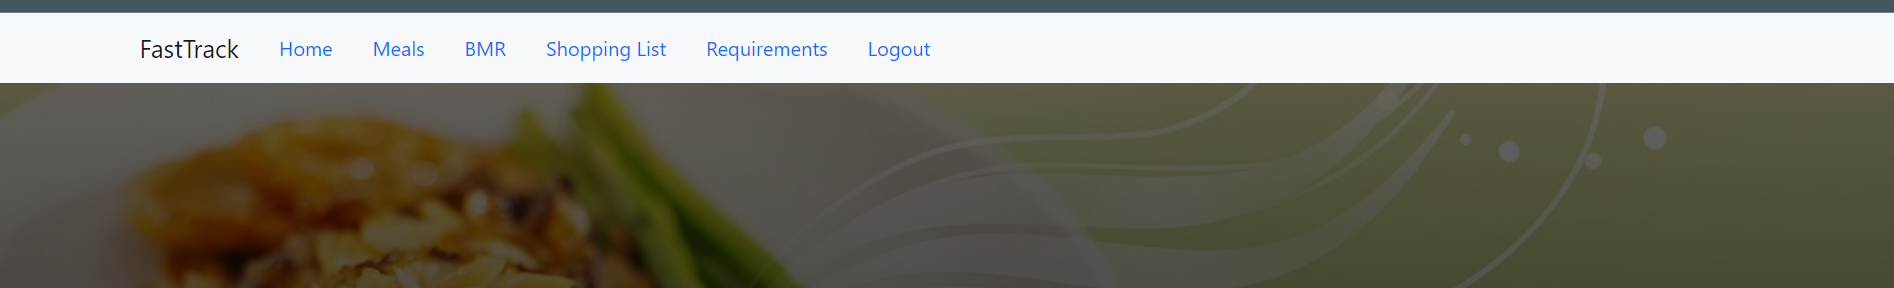
\includegraphics[width=\textwidth]{img/navbar.png}
    \caption{Navigation Bar}
    \label{fig: Image of Navigation Bar}
  \end{figure}
\end{center}

\subsection{Jumbotron}

The Jumbotron component is a simple HTML jumbotron that we use in our home (dashboard) page, the component contains a background image and a search bar for the meal landing component, where users can search for specific meals (recipes) based on the string of characters the user has added in the search bar, after the user clicks the search button then only meals matching the string of characters are displayed on the page.

\begin{center}
  \begin{figure}[H]
    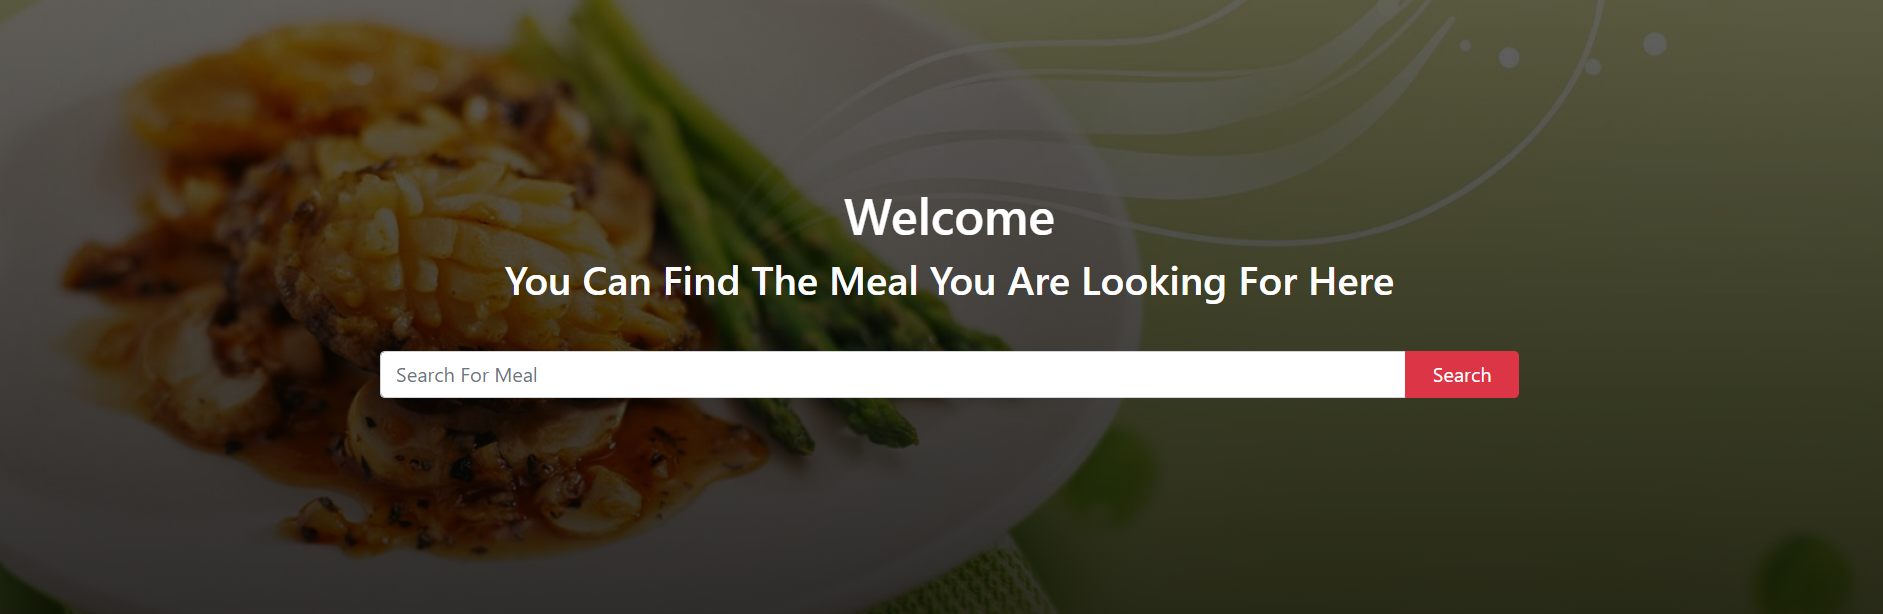
\includegraphics[width=\textwidth]{img/jumbotron.png}
    \caption{Jumbotron}
    \label{fig: Image of Jumbotron}
  \end{figure}
\end{center}

\subsection{404}

the 404 component is an error page for the application where any 404 (Not Found) client-side errors are handled. If a user attempts to enter an address of the application that does not exist or when a request is not found, the user will be redirected to this very page where the an error message is displayed. 

\section{Server Side}

In this section, I will discuss the libraries and frameworks used to develop the back end of my web application.

\subsection{ExpressJS}

ExpressJS is server-side, back end web application framework that is used for NodeJS needed to write simple and secure applications. ExpressJS is essential as it provides easy routing for requests sent by clients and provides middleware needed to make decisions to give correct responses for requests sent. There is also the advantage of formatting the data into a JSON-esque format, making it easy for users to read.

\subsection{NodeJS}

NodeJS is a open source, cross platform back end JavaScript run time environment, running the JavaScript code outward of the browser. NodeJS was essential in building the back end (server side) of my application as it provided features making it simple to understand and use. As I previously mentioned it is cross-platform meaning it can be used by many different languages which helped when using which is also an advantage.

\subsection{Mongoose}

Mongoose is a JavaScript library that creates a connection between MongoDB and the Express web application framework. Mongoose was essential in using my CRUD (create, read, update and delete) operations as well as developing my database schemas and also in performing search functionality by finding data using an 'id' parameter.

\begin{minted}{JavaScript}
const mongoose = require('mongoose');
const bcrypt = require('bcrypt');
const jwt = require('jsonwebtoken');
const userSchema = new mongoose.Schema({
  email: {
    type: String,
    required: true,
    unique: true
  },
  password: {
    type: String,
    required: true,
  },
  token: {
    type: String
  },

  favorites: {
    type: [String]
  }
})

userSchema.pre('save', async function (next) {
  const user = this;
  if (user.isModified('password')) {
    user.password = await bcrypt.hashSync(user.password, 10);
  }
  next();
})

userSchema.statics.findByCredentials = async function (email, password) {
  const user = await User.findOne({email});
  if(!user) {
    throw new Error('Invalid Credentials')
  }
  const passwordMatch = await bcrypt.compareSync(password, user.password)
  if(!passwordMatch) {
    throw new Error('Invalid Credentials')
  }
  return user;
}

userSchema.methods.generateToken = async function() {
  const user = this;
  const token = await jwt.sign({_id: user._id}, 
  "mealsSecret", {expiresIn: "365d"});
  user.token = token;
  await user.save();
  return token;
}

userSchema.methods.toJSON = function() {
  const user = this;
  const userObject = user.toObject();
  delete userObject.password;
  delete userObject._id;
  return userObject;
  
}

const User = mongoose.model('User', userSchema);
module.exports = User
\end{minted}

\section{User Interface and User Experience}
In this section, I will discuss how I designed, why I chose the the user interface of my application and discuss how I tested the user experience of my application.

\subsection{Evaluation}

The User Experience, sometimes referred to as the 'UX' or 'UE' is the design process of what the experience will be with how users interact with a select product, service or system. This process is typically followed by all or a majority of companies and design teams when a product, service or system has been developed to test a user or customers satisfaction with said product, service or system regarding usability, functionality and user interface. User Experience is a mixture of statistical study, product design and development, and strategies. User Experience is obviously always going to be personal and subjective as a certain user may be satisfied with a product, service or system for specific reasons while another user may now for those same reasons or for other reasons.\\ \\
To user experience of the application is necessary as most application in this field are either not aesthetically pleasing or too complicated for users to understand. In the evaluation process of my user experience, I presented my application to a select few people, experienced software engineers, graduate students and users of apps in this same field, where I collected data and information based on how they felt about using the app and if there was any changes they would make with their overall experience in using the application, any changes were written down and taken into consideration on whether I would make later changes during the development process of the application.

\section{Database}

In this section, I will discuss how I set up and implemented the database(s) of my application.

\subsection{MongoDB Atlas}

MongoDB Atlas as previously discussed, is a free, multi-cloud, database service that I used to develop my database schema for my database and store all the collection of data from my application, this data included information such as user details (emails and passwords), meals and ingredients. This was set up on the server side of my application and used Bcrypt to encrypt specific information in our database. Application as popular as Facebook, Twitter and Google all use MongoDB Atlas for this very purpose. I discussed earlier why I decided to use MongoDB Atlas for specific reasons such as scalability, accessibility and due to it's high performance level for large scale application.

\section{Architectural Styles and Patterns}

In this section, I will discuss the architectural styles or patterns, how I implemented architectural styles and patterns into my application. 

\subsection{REST}

To ensure that my application met all the RESTful architecture constraints and guidelines that were required, I'll explain how I approached each constraint as follows:

\begin{itemize}
    \item \textbf{Uniform Interface:} To ensure that this constraint was followed, as explained before I used HTML and CSS to design the interface of my application. I ensured that each HTML and CSS class that I used for all the components all matched.
    \item \textbf{Client-Server:} To ensure that this constraint was followed, I used Axios which is a promise-based HTTP Client for NodeJS and the browser, this allowed me to send a message (GET, POST, DELETE, etc.) from the server to the client and in return the server will receive a message response from the client and both the server and the client acted independent from one another.
    \item \textbf{Stateless:} To ensure that this constraint was followed, I used JSON Web Token which is a proposed internet standard for share security information between the client and a server. This allowed the user to store and secure all information from messages sent and received in the event of the server crashing or failing. JSON Web Token also worked in conjunction with Axios to perform this task. 
    \item \textbf{Cacheable:} To ensure that this constraint was followed, as I mentioned before I used JSON Web Token to work with Axios which allowed me to send, edit and receive information as well as securing the system and processes.
    \item \textbf{Layered System:} To ensure that this constraint was followed, I followed the guidelines and create a layered system, creating a three layered system, the first layer we deployed our API (TheMealDB API) using CORS, the second layer we used to store data using JSON Web Token and the third layer we used to authenticate requests using Axios.
\end{itemize}

\section{Encryption}

In this section, I will discuss how I set up the hashing password function for the user details in the User database schema for my application.

\subsection{Bcrypt}

To protect user details and information I used the JavaScript library 'Bcrypt', this library provides a password-hashing function which we used to encrypt all users password that have registered to the application, this encryption is generated as soon as the user enters their details in the registration form. I applied this as most application nowadays provide security features to prevent an attack by any unwelcome users and to create an application that follows the government cyber security guidelines.

\begin{minted}{JavaScript}
userSchema.pre('save', async function (next) {
  const user = this;
  if (user.isModified('password')) {
    user.password = await bcrypt.hashSync(user.password, 10);
  }
  next();
})

userSchema.statics.findByCredentials = async function (email, password) {
  const user = await User.findOne({email});
  if(!user) {
    throw new Error('Invalid Credentials')
  }
  const passwordMatch = await bcrypt.compareSync(password, user.password)
  if(!passwordMatch) {
    throw new Error('Invalid Credentials')
  }
  return user;
}
\end{minted}

\subsection{JSON Web Token}

To ensure all connections to the application are secure I used JSON Web Token which is known as the proposed internet standard for creating data. JSON Web Token generates tokens that provide a private secret or public/private key. For example. If the client has logged into the application, the server will generate a token which the client can the use to prove that their connection to ther server is legitimate.

\begin{minted}{JavaScript}
userSchema.methods.generateToken = async function() {
  const user = this;
  const token = await jwt.sign({_id: user._id}, "mealsSecret", 
  {expiresIn: "365d"});
  user.token = token;
  await user.save();
  return token;
}
\end{minted}

\chapter{System Evaluation}

\section{Overview}

In this section, I will give a quick overview on my evaluation of my project against the objective I set out for myself in the 'Introduction'.\\ \\
During the process of creation my application, as previously mentioned in the 'Introduction' chapter, I crafted the key objectives I set out for myself to follow and accomplish.

\section{Behavior, Robustness and Structure}

In this section, I will discuss how I tested the behavior and robustness of my web application.

\subsection{Testing}

For this project, I used two different types of testing to develop this application, Unit Testing and Acceptance Testing. The unit testing was utilized to verify the code and notify us if it is failing and acceptance testing tells you whether your code is working and complete. I used the two different types of testing framework (Selenium and Unit.js), during the development I discovered there was undetected bugs in my code coming from the software being outdated. Both Selenium and Unit.js proved extremely useful as during this development as every time I added new code to my application, these tests ensured that this code always worked intended.

\subsection{Stability}

Stability in terms of applications is the measurement of application health and user experience. App stability can be measured in two general ways: either as a percentage of app sessions that don't crash or encounter an unhandled exception, or as the percentage of regular daily users who do not experience an error. I have tested the application vigorously to ensure that the app is always stable, when the app seemed to be even slightly unstable, I pinpointed what the issue may be by running tests and attempted to solve the problem. The application isn't completely free of errors as there are only a few errors that the application runs into at time including:

\begin{itemize}
    \item The total of the shopping list component won't always update on the first attempt but when it is updated a second time it will work just fine.
    \item Users may have to click the log in button multiple times when logging in but this has issue has only occured on very few occasions.
\end{itemize}

It is rare to find large scale applications that are free of all bugs and even with these small errors in my application, this app still runs and functions as intended and maintains it's stability.

\section{Performance Benchmarks}

In this section, I will discuss how I measured the performance of a my application against other application in the same field.

\subsection{Scope}

The scope refers to requirements specified to achieve the end result specifically what the project is to accomplish and a description of what the end result should be or accomplish. The main part regrading the scope of the application is the software quality, the quality is connected to the time invested into the application as the amount of time invested in specific tasks set out to complete will define the overall quality of the product, certain tasks will take longer than other to complete but this may mean this task will be completed exceptionally. I created a single page, large scale application meaning the scope of the project was quite big and a large number of tasks had to be completed.

\subsection{Time}

I considered many different techniques to produce my product in an estimated time period, the method I chose to go with is using Agile Methodology using Atlassian to set up two week sprints to identify tasks needed to produce the deliverables documented, I broke down the tasks needed to be carried out by referring to the key objectives I set out for myself and then set up these sprints before I started developing the application so I had a list of tasks, the tasks are also prioritized, dependencies between tasks are identified, and this information is documented in a project schedule. Once the two week period was up for the sprint was up, I reviewed all the tasks that were to be completed and checked if this select task was complete to ensure the product was fully developed in an estimated time period, I set up eight sprints in regard to developing my application (all other sprints were in regard to my dissertation) meaning the estimated time period I set for myself was 4 months.

\section{Outcomes}

In this section, I will discuss how I measured the outcome of my application against the set objectives.

\subsection{Multi-User Web Application}

I have created a single-page, web application that can be accessed by multiple users simultaneously, I tested with other professionals that the application and all it's pages work as intended synchronously especially the API that I used as their were worries any client-server requests and responses regarding the API work across multiple machines. All pages and components fulfill their purpose while being accessed simultaneously, this is due to the use of JSON Web Token where JSON Web Token generate tokens that provide a private secret or public/private key for user sessions and one user will not affect another users session.

\subsection{Functionality}

The application achieves many of the functionality of the components that I set out for myself including:

\begin{itemize}
    \item The application performs CRUD functionality by adding, retrieving, editing and deleting meals from the users meal listing component.
    \item The application provides a calories calculator calculates the user BMR (Basic Metabolic Rate) and calories needed based on the users details.
    \item The application provides a shopping list component that also performs CRUD functionality where users can add, edit and delete ingredients that they need to purchase.
    \item The application implements ChartJS where we created a table of charts where every chart represents the percentage of the total calories of different diets and a link to further information on each diet.
\end{itemize}

\subsection{Data Security}

The application is password encrypted and user sessions are secured using both Bcrypt and JSON Web Token. User passwords are hashed by using Bcrypt which is a password-hashing function where as soon as a new user is registered into the application the password is automatically encrypted to prevent any cyber security attacks and follow modern guidelines. We have previously discussed the use of JSON Web Token as I implemented this to generate tokens that provide a private secret or public/private key for user sessions to ensure all information stored in a user session is not shared publicly.

\subsection{REST}

I followed all REST constraints when developing my application, the application has a uniform interface, the app is both stateless and cacheable, it is client-server independent and has a layered system. When CRUD (Create, Read, Update and Delete) is performed, all data is stored in our database (MongoDB). As we previously mentioned, the app is both stateless and cacheable, it is stateless as we used JSON Web Token the user to store and secure all information from messages sent and received in the event of the server crashing or failing and it is cacheable also using JSON Web Token and Axios to to send, edit and receive information as well as securing the system and processes.

\section{Limitations}

In this section, I will highlight any limitations or opportunities in my approach or in the technology.

\subsection{Performance}

This is a large scale application and the application is connected to the web browser which in turns means the app size will increase, the impact of this can be seen in the performance of a web application as a large scale web application is slower than a native application. Web applications will possibly never replace mobile apps and it’s very likely that a web app will operate at a slightly slower speed than one that is hosted on a server locally. PWAs (progressive web applications) definitely try to mitigate this side effect, but there’s no veritable evidence that they have successfully eliminated this disadvantage altogether.

\subsection{Updating}

Continuously updating the software I was using became a limitation further down the line in the development of my application, as I was progressing with the development of my application, certain software that I used at the start of the Software Development Life Cycle (SDLC) would become outdated or become vulnerable to security issues which meant I would have to update the software but at the same time continuous updating could affect the code I was using as certain pieces of code could also become outdated and no longer used by this software. To solve this issue, I updated all the software that was outdated in a two week sprint and tested all the code afterwards, pinpointed any errors that were detected and researched the alternatives to replace this code to stick with the updated software.

\subsection{Internet Dependence}

This application is internet dependent and an internet connection is compulsory when running a web application which is very limiting in regards to most application nowadays and there are still many parts of the world where internet is not accessible, without a reliable internet connection you cannot either browse the web or run the application. Due to the software I was using, namely the MERN Stack (MongoDB, ExpressJS, ReactJS, NodeJS) there wasn't a way I could make this application non-internet dependent. 

\chapter{Conclusion}

\section{What Were The Learning Outcomes}

In this section, I will discuss what I learned throughout the development of my application.

\subsection{Project Management}

Project management was the most important lesson I gained as I intend to move deeper into the world of software engineering where working with other developers, project management is gong to be the most important factor while working on a software project or product. During the development lifecycle of the application, I gained project management skills such as problem solving, time management and risk management needed to initiate, plan, and execute a project, the only difference being project management usually is learned from working with a team of people as opposed to working by yourself.

\subsection{Scope}

During the planning phase of the application, I learned a lot especially attempting to gauge what is the correct size of the scope for this project. I went through countless brainstorming sessions of what my project was going to be, after several concepts and ideas that fell to the wayside (due to not believing the scope was big enough), I encountered an idea that I thought would work and if the initial ideas scope wasn't large enough then I could still expand upon it. \\ \\
While encountering this issue, scope creep was another issue that I encountered when dealing with the scope of the project but this was an issue during the developmental phase (coding). Scope creep in project management refers to changes, continuous or uncontrolled growth in a project’s scope, at any point after the project begins. It was difficult to continuously combat scope creep due to the number features and improvements I planned to add to my application, this lead to features (see Incomplete Ideas) that I wished to implement being left out due to time constraints and focus on the main features I had already set out to complete.\\ \\
After completing this application, I learned the heavy disadvantages that come with scope creep as it forced me to rush the focus certain features at times but at the same time it informed me on how to tolerate this issue in any upcoming projects, by assigning a weight to each task or feature, the heaviness of the weight regarding it's significance.

\subsection{Objectives}

When I set out the objectives for myself to be completed, I planned to do research on each of these objectives to gain knowledge of what I am trying to accomplish, for the most part I had to understand applications and how they work. For example, one of my objectives was to create a large scale, multi-user, functioning web application that can be accessed, in doing this I had to research what is a web application and how does it different from other types of applications, e.g. mobile application, I also had to gain knowledge on what makes an application to be considered large scale.

\subsection{MERN Stack}

I gained much knowledge pertaining to the MERN Stack and the four key technologies that make up the stack, I had little experience with each of these technologies but after building this application, I gained so much experience and knowledge with these frameworks and learning these technologies helped me gain the skill of learning new frameworks. ReactJS provided me with many libraries to implement functionality such as saving user sessions, encrypting passwords or drawing charts, ReactJS to me was more appealing than using an alternative framework (AngularJS). ExpressJS and NodeJS helped me develop the back end of my application and run on a machine rather than a browser. MongoDB really taught me so much about the inner workings of databases and how they are operated and used.

\section{What I Did Different}

In this section, I will discuss how my application differs from meal planning applications nowadays.

\subsection{Shopping List}

During the research phase of my application, I viewed the most popular meal planning applications and compared them all and I noticed that while it is easy to develop an app to sort out meals that a person will eat in a day, these apps don't provide any type of organization for the ingredients these meals need. I believe this feature is necessary as sorting out what ingredients are needed for the day provides many advantages such as cost effectiveness as it impacts the cash you spend and it is an easy way to track calories and weight gain. I created this feature using a simple React Hook Form that I connected to our database where users can add, edit and delete the ingredients and the quantity of said ingredient.

\subsection{Calculator}

We discussed earlier on the addition of this BMR (Basic Metabolic Rate) and Calories Needed Calculator that is used to calculate both the BMR and calories needed by the user based on information the user provides (age, gender, weight, height, etc.). This feature was actually a late idea in the planning phase and came just before I was moving into to the coding stage of my application, after vigorous research I came up with the idea that a calculator to calculate both the BMR and calories needed was positive for the application and works well the concept of the application and meal planning and weight watching go hand in hand, this feature is something you will not find in meal planning apps but I believe this is something that is important to add to meal planning apps in the future.

\subsection{Dietary Information}

This is a simple feature that I didn't notice any other applications in this dame field provided, where the user is provided with links containing information on various diets in the world that a user may want to either follow or might want to look into. I did this in conjunction with the dietary charts (I will discuss this feature later) and I provided various chart, each containing a specific diet with a hyperlink that navigates the user to a site with much more information on this specific diet.

\subsection{Dietary Charts}

I previously mentioned above how my Dietary Charts feature worked in conjunction with the Dietary Information feature. I created a page full of a table of pie charts, each chart represented an official diet (vegan diet, ketogenic diet, low-carb diet, etc.), the data of each chart are based on the percentage of food intake of different 3 or 4 food groups (Fruits \& Vegetables, Carbohydrates, Proteins and Fats) where if the user selects to use this diet they must confine to this food intake regimen. I created this feature by simply using HTML Tables to help set up the table to accommodate the charts and the JavaScript library chart.js to create each chart, I pondered the idea to use an API and GraphQL to represent the data but in the end I came to the conclusion that using chart.js and setting the data manually was the easier option.

\section{How Did Testing and Methodology Help}

In this section, I will discuss how the addition of testing and methodology helped me throughout the development of my application.

\subsection{Testing}

The use of testing frameworks was needed in the development of this application, there are many different roles needed in the software development lifecycle albeit the UX/UI designer, software developer, project manager but one role that is very important is the tester, in doing this project I had to take on all roles each one and while developing code for the application, the use of testing helped me to improve code quality as I would continuously test my application to check if the code works as intended or if any new code addition affects the previous code that existed allowing me to refactor this code once every check is complete. This very advantage helped me to complete many of the components and features that I set to create for the application as instead of reflecting on how far can I go to make this component or feature as great as I had in my mind, I decided it was better for the feature to pass all tests instead.

\subsection{Methodology}

The use of Agile Methodology (specifically Atlassian) was exponentially important in the development of this application, it was the most important practice I could have used to maintain the project management of the development of the application, it was the use of sprints is what helped me complete this application in the time frame that I wished to complete it in. The sprints were designed to be completed in two week periods where in each sprint I set out a list of objectives that had to be completed (if any errors/faults occurred they were to be noted and dealt with later) and this allowed me to implement all functionality and features with the least amount of fault and as smoothly as possible. The issues that occurred in any sprint was documented in a backlog where I would check the error and add to another sprint to be completed.

\section{What Changes Would I Make}

In this section, I will discuss if there are any changes I would have made to my application after now completing it.

\subsection{Planning Phase}

The planning phase had a few ups and downs that could have been avoided while planning for all areas of the project, reflecting on this time I felt that I could have put even more thought into this project during this phase, some issues I encountered during this phase included continuously changing what the project was going to be and fleshing out better ideas for functionality. I kept changing what the concept of the was going to be due to either not fully liking the idea or being over concerned with if the scope of this project was large enough, this could have been prevented if I had put more thought and effort in the planning phase of this project. During the development of my application, there were many features that I wished to add to my application but didn't come to fruition and in return there was features that I did implement into my application that were not not thought through to the best of my ability, if I had planned these features better these features would have been done without error and may have been more advanced than the current version. Apart from the above mentioned issues, the planning phase in my eyes was a success and went as intended to.

\subsection{Incomplete Ideas}

I previously mentioned how I had features that I wished to implement into my application but due to some poor planning techniques these ideas could not reach fulfillment, one idea was to add another API to my application that would allow users to view the different restaurants that are in their region/area using a Google Map like feature. This idea I was very excited to implement and I taught it would have been a great feature to work with the application but due to poor planning this could not emerge as intended.

\section{Summary}

In this section, I will give a brief summary and some last words for this dissertation regarding my project.

\subsection{In Conclusion}

In conclusion, this module as well as my four years of learning at GMIT, assisted in helping me gain so many skills and qualities of a software developer, as I used these skills to create a multi-user, web application, an application that I out my heart and soul into and one that I am very proud of. I learned to think like a software developer when developing projects, focusing on aspects such as the User Experience, User Interface, planning, testing, documentation and so on but most important it taught me to understand quality of code and how to differentiate between good and bad code. \\ \\ 
I would like to send a personal thank you to every single lecturer that has played a role in my four year journey of software development, I wish I could name them all but there won't be enough space in this report, your distribution of knowledge in the field of computer science helped me gain and improve the necessary skills needed in this field and provided me with a protective and engaging environment to do so which has helped prepare me for the future. I can only express how much your lessons, teachings and the experience you provided as a whole have taught me a lot about myself as a person and what I would like my future to become. \\ \\ 
Thank you so much for reading through this long dissertation and looking at my project, it has been long but adventurous journey where I have learned various fields in regards to computer science. When I first decided to follow this course, I didn't know much or anything about coding but I always enjoyed learning about computers and I was under the notion that software development involved just writing pieces of code that function together but I now see the bigger picture where planning, time management, risk management, scheduling, problem solving and so many more factors are the main priorities when supplying a customer with a software product.\\ \\ 
Finally, I wish to also like to give some personal praise to my final year project supervisor, Dr. Joseph Corr for really giving me so much help and guidance throughout this whole process, whether it was helping me brainstorm ideas, suggesting the use of Agile Methodology and guiding me through the design phase of my application, it was with his helping hand that everything went as smooth as it did and for that I am forever thankful.\\ \\ 
Thank you to all reviewing this dissertation and observing my code, I hope this is to your normal high standard and please view the hyperlinks provided by myself to all further documentation in the Appendix section coming up next. My name is Emmanuel Osabuehien and this is my final year project. Farewell.

\begin{appendices}
\begin{itemize}
\item \href{https://github.com/Emmanuel-Osabuehien/AppliedProjectMinorDissertation}{Click This Link To View GitHub Repository Used To Develop This Project}
\item \href{https://github.com/Emmanuel-Osabuehien/AppliedProjectMinorDissertation/tree/main/meal-planning-system}{Click This Link To View The Source Code Of The Project On GitHub}
\item \href{https://github.com/Emmanuel-Osabuehien/AppliedProjectMinorDissertation/tree/main/dissertation}{Click This Link To View The Dissertation Files On GitHub}
\item \href{https://g00373559.atlassian.net/jira/software/projects/MPRO/boards/4}{Click This Link To View The Agile Board Used To Develop The Project}
\end{itemize}
\end{appendices}